\documentclass[%
	11pt,
	a4paper,
	utf8,
	%twocolumn
		]{article}	

\usepackage{style_packages/podvoyskiy_article_extended}


\begin{document}
\title{Заметки по машинному обучению и анализу данных. Том 2}

\author{\itshape Подвойский А.О.}

\date{}
\maketitle

\thispagestyle{fancy}

Здесь приводятся заметки по некоторым вопросам, касающимся машинного обучения, анализа данных, программирования на языках \texttt{Python}, \texttt{R} и прочим сопряженным вопросам так или иначе, затрагивающим работу с данными.


\shorttableofcontents{Краткое содержание}{1}

\tableofcontents

\section{Приемы работы с библиотекой анализа временных рядов ETNA}

\subsection{Перекрестная проверка на временных рядах}

Перекрестную проверку с расширяющимся окном (или на скользящем окне) в бибилотеке ETNA можно выполнить с помощью метода \verb|.backtest()|. Этот метод возвращает три кадра данных: кадр данных с метриками по каждой тестовой выборке перекрестной проверки, кадр данных с прогнозами и кадр данных с временными метками обучающего и тестового поднаборов данных.

В перекрестной проверке расширяющися окном количество наблюдений, использованных для обучения в каждой итерации, растет с числом итераций, предоставляет все больший объем данных для обучения.

\begin{figure}[h]
	\centering
	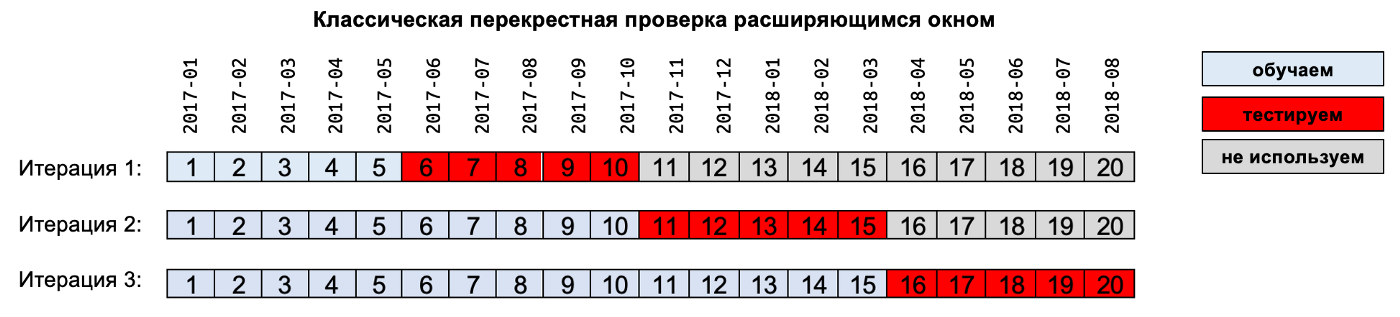
\includegraphics[scale=0.3]{figures/cross_val_ts.png}
	\caption{ Перекрестная проверка на временном ряду \emph{расширяющимся} окном }\label{fig:cross_val_ts}
\end{figure}

Для тестирования мы каждый раз берем совершенно новые более поздние наблюдения. Обучающая выборка прирастает на количество наблюдений, равное горизонту прогнозирования.

При необходимости обучение модели в каждом разбиении можно сделать последовательным, используя в каждой итерации для обучения фиксированное количество наиболее свежих (поздних) наблюдений, предшествующих точке разбиения. Таким образом, в каждой новой итерации мы будем обучаться на более свежих данных, обучающая выборка каждый раз сдвигается вперед по временной оси (обычно на горизонт прогнозирования) и такой способ проверки называют перекрестной проверкой скользящим окном (sliding/rolling window).

\begin{figure}[h]
	\centering
	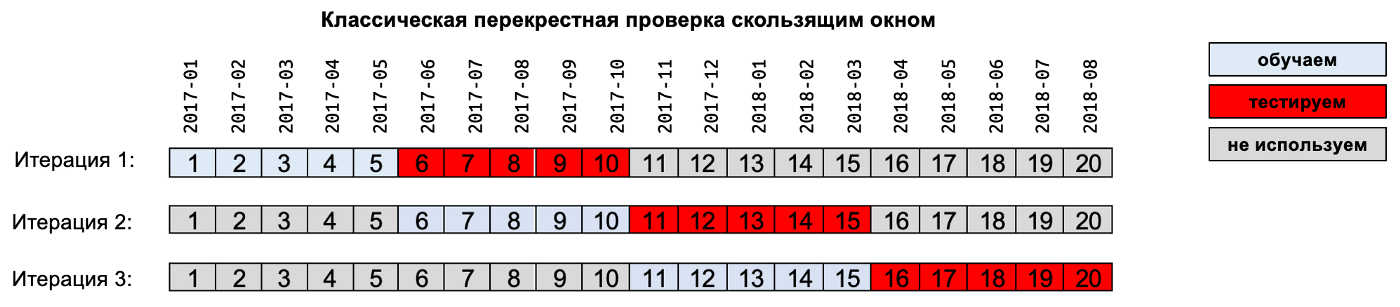
\includegraphics[scale=0.3]{figures/cross_val_rol_ts.png}
	\caption{ Перекрестная проверка \emph{на скользящем} окне }\label{fig:cross_val_rol_ts}
\end{figure}

С каждой итерацией обучающая выборка использует все более свежие наблюдения, при этом для тестирования мы каждый раз берем совершенно новые более поздние наблюдения. Размер обучающей выборки остается неизменным, поэтому в ETNA этот вид проверки назван \verb|constant|.

NB При выполнении перекрестной проверки для временных рядов полезно помнить ряд правил:
\begin{itemize}
	\item Размер тестовой выборки, как правило, определяется горизонтом прогнозирования, а тот в свою очередь определяется бизнес-требования. Если вы предсказываете на 14 дней вперед, то и тестовая выборка должна включать 14 более поздних наблюдений.
	
	\item Размер тестовой выборки остается постоянным. Это значит, что метрики качества, полученные в результате вычислений прогнозов каждой обученной модели по тестовому набору, будут последовательны и их можно объединять и сравнивать.
	
	\item Размер обучающей выборки не может быть меньше тестовой выборки.
	
	\item Если данные содержат сезонность, обучающая выборка должна содержать не менее двух полных сезонных циклов (правило $ 2L $, где $ L $ -- количество периодов в полном сезонном цикле, необходимое для инициализации параметров некоторых моделей, например, для вычисления исходного значения тренда в модели тройного экспонециального сглаживания), учитывая уменьшение длины ряда при выполнении процедур обычного и сезонного дифференциирования.
	
	\item Если применяются переменные -- лаги, разности на лагах, скользящие статистики, то каждый раз для получения значений в тестовой выборке используются только данных обучающей выборки.
\end{itemize}

Перекрестную проверку расширяющимся окном можно модифицировать так, чтобы обучающая выборка прирастала на количество наблюдений меньше горизонта прогнозирования и тогда в тестовую выборку попадут наблюдения, уже попадавшие в тестовую выборку на предыдущей итерации. Это позволяет управлять скоростью обновления модели, лучше выявлять аномальные, нетипичные наблюдения, которые плохо предсказываются, точнее определить момент ухудшения качества модели.

\begin{figure}[h]
	\centering
	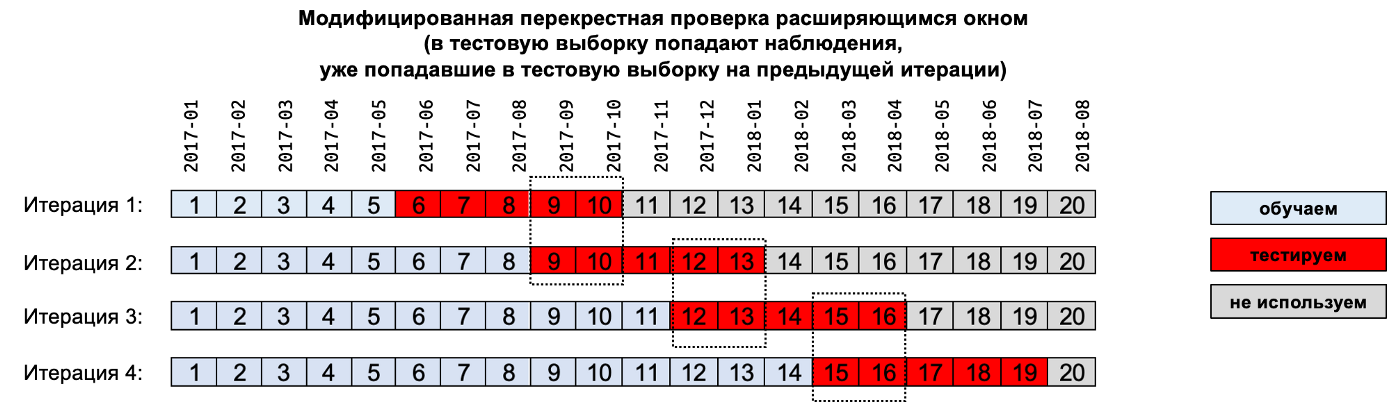
\includegraphics[scale=0.3]{figures/cross_val_expand_ts.png}
	\caption{ Модфицированная перекрестная проверка расширяющимся окном }\label{fig:cross_val_expand_ts}
\end{figure}

Перекрестную проверку скользящим окном тоже можно модифицировать так, чтобы обучающая выборка сдвигалась вперед не на весь горизонт прогнозирония, а на половину или на треть, и тогда в тестовую выборку попадут наблюдения, уже попадавшие в тестовую выборку на предыдущей итерации. Это позволяет управлять скоростью обновления модели, лучше выявлять аномальные, нетипичные наблюдения, которые плохо предсказываются, точнее определять момент ухудшения качества модели.

\begin{figure}[h]
	\centering
	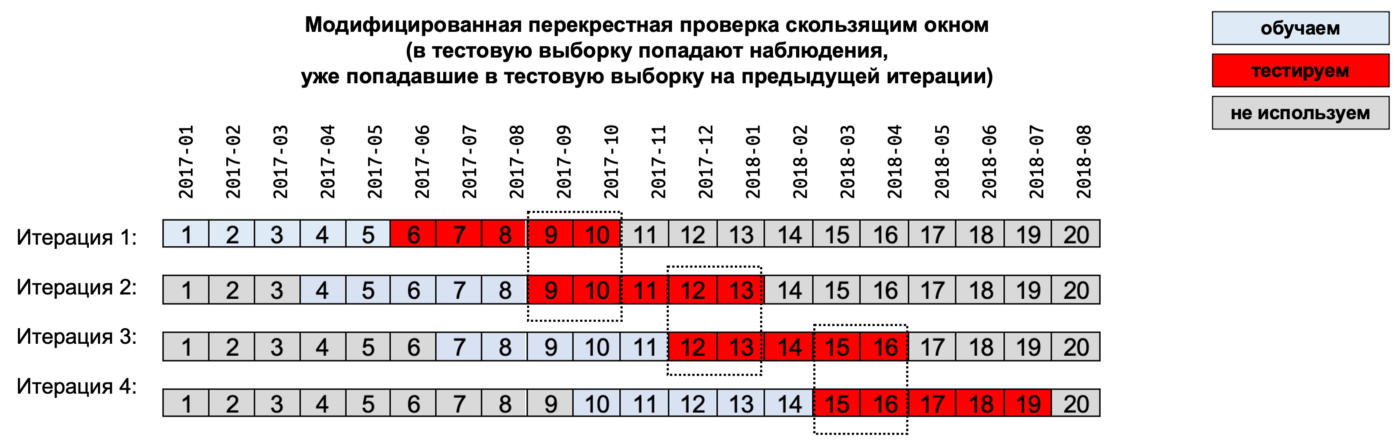
\includegraphics[scale=0.3]{figures/cross_val_rol_modif_ts.png}
	\caption{ Модфицированная перекрестная проверка скользящим окном }\label{fig:cross_val_rol_modif_ts}
\end{figure}

Однако, в библиотеке ETNA и библиотеке scikit-learn с помощью класса TimeSeriesSplit нельзя корректно реализовать вышеописанные модификации.

При использовании перекрестной проверки расширяющимся окном модель в большей степени нацелена на обнаружение глобальных паттернов и менее склонна к изменениям, т.е. более консервативна. При использовании перекрестной проверки скользящим окном используется меньше данных, модель быстрее меняет поведение, т.е. менее консервативна. В ситуации, когда вы уверены, что процесс, генерирующий данные, изменился или неоднократно менялся в течение периода, охватывающего исторические данные, используйте перекрестную проверку скользящим окном.

Для рынков товаров с низкой вовлеченностью (товаров повседневного спроса), в ситуации, когда вы уверены или у вас есть доказательства, что процесс, генерирующий данные, остается неизменным или претерпевает несущественные изменения, перекрестная проверка расширяющимся окном может быть более полезна.

\remark{
Важно помнить, что во временных рядах \emph{перекрестная проверка}, которую вы применяете, является \emph{прообразом} вашей \emph{производственной системы}. Если вы применяли для валидации перекрестную проверку расширяющимся окном, то и в производстве вы должны обучать модель на обучающей выборке возрастающего объема и обновлять в том же темпе, что обновляли в ходе перекрестной проверки (на весь горизонт прогнозирования, на половину горизонта и т.д.)
}

Наконец, поскольку в рамках перекрестной проверки расширяющимся окном мы на каждой итерации обучаем модель на выборке все большего объема, при использовании моделей на основе градиентного бустинга это может потребовать коррекции темпа обучения, количества деревьев и максимальной глубины. 

\subsection{CatBoost. Базовая модель с конструированием признаков}

В ETNA есть два класса-обертки над классом \texttt{CatboostRegressor}: \texttt{CatBoostModePerSegment} и \texttt{CatBoostModelMultiSegment}. Разница заключается в том, что класс \texttt{CatBoostModelPerSegment} обучает отдельную модель для каждого сегмента, а класс \texttt{CatBoostModelMultiSegment} -- одну модель для всех сегментов.

Для создания признаков можно использовать классы-трансформеры:
\begin{itemize}
	\item \texttt{LagTransform} для генерации лагов,
	
	\item \texttt{MeanTransform} для вычисления скользящего среднего по заданному окну.
\end{itemize}

\remark{
Ширина скользящего окна не должна превышать горизонт прогнозирования
}

С помощью параметра \verb|in_column| класса-трансформера задаем переменную, которую нужно преобразовать или на основе которой нужно создать признаки (по умолчанию этой переменной будет переменная \texttt{target}). С помощью параметра \verb|out_column| (этот параметр есть у всех классов-трансформеров, создающих признаки) можно задать имена генерируемых переменных.

Для более надежной оценки качества модели следует восопользоваться \emph{перекрестной проверкой расширяющимся окном} с помощью класса \texttt{Pipeline}.

Создадим список преобразований. В данном случае он включать формирование лагов и скользящего среднего на каждой итерации перекрестной проверки.

\begin{lstlisting}[
style = ironpython,
numbers = none
]
lags = LagTransform(in_column="target", lags=list(range(8, 24, 1)), out_column="lag")
mean8 = MeanTransform(in_column="target", window=8, out_column="mean8")
transforms = [lags, mean8]
\end{lstlisting}

Теперь создаем конвейер для выполнения перекрестной проверки расширяющимся окном, передав в него модель, список процедур формирования признаков (лагов и скользящего среднего) и горизонт прогнозирования
\begin{lstlisting}[
style = ironpython,
numbers = none
]
model = CatBoostModelMultiSegment()
model.fit(train_ts)

pipeline = Pipeline(
    model=model,
    transforms=transforms,
    horizon=HORIZON,
)
# перекрестная проверка расширяющимся окном
metrics_df, _, _ = pipeline.backtest(
    ts=ts,
    mode="expand",
    metrics=[smape],
)
\end{lstlisting}

Класс \texttt{Pipeline} можно использовать для перекрестной проверки сразу нескольких моделей
\begin{lstlisting}[
style = ironpython,
numbers = none
]
# задаем конвейер преобразований для модели наивного прогноза
naive_pipeline = Pipeline(
    model=NaiveModel(lag=12), transforms=[], horizon=HORIZON)
# задаем конвейер преобразований для Prophet
prophet_pipeline = Pipeline(
    model=ProphetModel(), transforms=[], horizon=HORIZON
)
# задаем конвейер преобразований для CatBoost
catboost_pipeline = Pipeline(
    model=CatBoostModelMultiSegment(),
    transforms=[LagTransform(lags=[8, 9, 10, 11, 12], 
    in_column='target')],
    horizon=HORIZON
)
# задаем список имен конвейеров
pipeline_names = ['naive', 'prophet', 'catboost']
# задаем список конвейеров
pipelines = [naive_pipeline, prophet_pipeline, catboost_pipeline]
# задаем пустой список метрик
metrics = []
# записываем метрики в список
for pipeline in pipelines:
    metrics.append(
        pipeline.backtest(
        ts=ts, metrics=[MAE(), MSE(), SMAPE(), MAPE()], 
        n_folds=3, aggregate_metrics=True
    )[0].iloc[:, 1:]
)

# конкатенируем метрики
metrics = pd.concat(metrics)
# в качестве индекса используем список имен конвейеров
metrics.index = pipeline_names
\end{lstlisting}

С помощью класса \texttt{VotingEnsemble} можно выполнить обучение и перекрестную проверку \emph{ансамбля моделей}. Веса моделей можно задавать с помощью параметра \texttt{weights}
\begin{lstlisting}[
style = ironpython,
numbers = none
]
# создаем экземпляр класса VotingEnsemble
voting_ensemble = VotingEnsemble(pipelines=pipelines, 
weights=[1, 2, 4], 
n_jobs=4)
# получаем метрики
voting_ensamble_metrics = voting_ensemble.backtest(
    ts=ts,
    metrics=[MAE(), MSE(), SMAPE(), MAPE()], 
    n_folds=3,
    aggregate_metrics=True,
    n_jobs=2
)[0].iloc[:, 1:]
voting_ensamble_metrics.index = ['voting ensemble']
\end{lstlisting}

С помощью класса \texttt{StackingEnsemble} можно выполнить \emph{стекинг}. Мы прогнозируем будущее, используя метамодель (линейную регрессию по умолчанию) для объединения прогнозов моделей в списке конвейеров. С помощью параметров \verb|final_model| можно задать метамодель. С помощью \verb|features_to_use| можно задавать признаки для метамодели
\begin{itemize}
	\item \texttt{None}: метамодель в качестве признаков может использовать прогнозы моделей конвейеров,
	
	\item \texttt{List}: прогнозы моделей конвейеров плюс признаки из списка (в виде строковых значений),
	
	\item \texttt{"all"}: все доступные признаки.
\end{itemize}

С помощью параметра \texttt{cv} задаем количество тестовых выборок перекрестной выборки (используем не для оценки моделей, а для получения прогнозов, которые станут у нас потом признаками).

Под капотом происходит примерно следующее. Допустим, запустили перекрестную проверку расширяющимся окном, получили 5 тестовых выборок, прогнозы каждой из модели конвейера в 5 тестовых выбоках стали признаками. Затем снова запускаем проверку расширяющимся окном, по этим признакам строим метамодель -- линейную регрессию, берем прогнозы в 3 тестовых выборках и усредняем
\begin{lstlisting}[
style = ironpython,
numbers = none
]
# создаем экземпляр класса StackingEnsemble,
# признаки - прогнозы конвейеров
stacking_ensemble_unfeatured = StackingEnsemble(
    features_to_use='None', pipelines=pipelines, 
    n_folds=10, n_jobs=4)
# выполняем стекинг
stacking_ensamble_metrics = stacking_ensemble_unfeatured.backtest(
    ts=ts, metrics=[MAE(), MSE(), SMAPE(), MAPE()], n_folds=3, 
    aggregate_metrics=True, n_jobs=2)[0].iloc[:, 1:]
stacking_ensamble_metrics.index = ['stacking ensemble']
stacking_ensamble_metrics
\end{lstlisting}

\subsection{Пользовательские классы для вычисления скользящих статистик}

Можно писать свои собственные классы для вычисления скользящих статистик и обучения моделей. Допустим, мы хотим использовать не только скользящие средние, но и скользящие средние абсолютные отклонения
\begin{lstlisting}[
style = ironpython,
numbers = none
]
# пишем класс MadTransform, вычисляющий скользящие
# средние абсолютные отклонения
class MadTransform(WindowStatisticsTransform):
    """
    MadTransform вычисляет среднее абсолютное отклонение
    (mean absolute deviation - mad) для заданного окна.
    """
		def __init__(
			self,
			in_column: str,
			window: int,
			seasonality: int = 1,
			min_periods: int = 1,
			fillna: float = 0,
			out_column: Optional[str] = None
		):
		"""
		Параметры
		----------
		in_column: str
		имя обрабатываемого столбца
		window: int
		ширина окна для агрегирования
		out_column: str, optional
		имя результирующего столбца. Если не задано, 
		используем __repr__()
		seasonality: int
		коэффициент сезонности
		min_periods: int
		Минимальное количество наблюдений в окне 
		для агрегирования
		fillna: float
		значение для заполнения значений NaN
		"""
		self.in_column = in_column
		self.window = window
		self.seasonality = seasonality
		self.min_periods = min_periods
		self.fillna = fillna
		self.out_column = out_column
		super().__init__(
		window=window,
		in_column=in_column,
		seasonality=seasonality,
		min_periods=min_periods,
		out_column=self.out_column 
		if self.out_column is not None 
		else self.__repr__(),
		fillna=fillna,
	)
	def _aggregate_window(
		self, series: pd.Series
	) -> float:
		"""Вычисляет mad для серии."""
		tmp_series = self._get_required_lags(series)
		return tmp_series.mad(**self.kwargs)
\end{lstlisting}

Теперь предположим, мы хотим использовать LightGBM вместо CatBoost. Нам понадобиться класс LGBRegressor и базовые классы библиотеки ETNA \texttt{Model} и \texttt{PerSegmentModel}.

Сначала надо написать ядро -- внутренний класс \verb|_LBGMModel|, в котором используется \texttt{LGBMRegressor}. Символ нижнего подчеркивания указывает, что данный класс будет использоваться внутри других классов. У класса \verb|_LGBModel| будут два метода \texttt{fit()} и \texttt{predict()}.

\begin{lstlisting}[
style = ironpython,
numbers = none
]
# пишем ядро - внутренний класс _LGBMModel,
# внутри - класс LGBMRegressor
class _LGBMModel:
	def __init__(
		self,
		boosting_type='gbdt',
		num_leaves=31,
		max_depth=-1,
		learning_rate=0.1,
		n_estimators=100,
		**kwargs
	):
		self.model=LGBMRegressor(
			boosting_type=boosting_type,
			num_leaves=num_leaves,
			max_depth=max_depth,
			learning_rate=learning_rate,
			n_estimators=n_estimators,
			**kwargs
		)
	def fit(self, df: pd.DataFrame):
		features = df.drop(columns=['timestamp', 'target'])
		target = df['target']
		self.model.fit(X=features, y=target)
		return self
		
	def predict(self, df: pd.DataFrame):
		features = df.drop(columns=['timestamp', 'target'])
		pred = self.model.predict(features)
		return pred
\end{lstlisting}

Вспомним, что мы можем строить отдельную модель для каждого сегмента и одну модель для всего набора (т.е. всех сегментов). Значит мы можем написать два класса. Начнем с класса, который будет строить отдельную модель для каждого сегмента. Назовем его \texttt{LGBModelPerSegment}. Для этого воспользуемся наследованием, нам понадобится базовый класс \texttt{PerSegmentModel}

\begin{lstlisting}[
style = ironpython,
numbers = none
]
# пишем класс LGBMModelPerSegment, который строит 
# отдельную модель LGBM для каждого сегмента
class LGBMModelPerSegment(PerSegmentModel):
	def __init__(
		self,
		boosting_type='gbdt',
		num_leaves=31,
		max_depth=-1,
		learning_rate=0.1,
		n_estimators=100,
		**kwargs
	):
		self.kwargs = kwargs
		model = _LGBMModel(
			boosting_type=boosting_type,
			num_leaves=num_leaves,
			max_depth=max_depth,
			learning_rate=learning_rate,
			n_estimators=n_estimators,
			**kwargs
		)
		super(LGBMModelPerSegment, self).__init__(
			base_model=model)
\end{lstlisting}

Теперь напишем класс, который будет строить одну модель для всех сегментов. Назовем его \texttt{LGBModelMultiSegment}. Для этого вновь воспользуемся наследованием, нам понадобится базовый класс \texttt{Model}

\begin{lstlisting}[
style = ironpython,
numbers = none
]
# пишем класс LGBMModelMultiSegment, который строит 
# одну модель LGBM для всех сегментов
class LGBMModelMultiSegment(Model):
	def __init__(
		self,
		boosting_type='gbdt',
		num_leaves=31,
		max_depth=-1,
		learning_rate=0.1,
		n_estimators=100,
		**kwargs
	):
		self.kwargs = kwargs
		super(LGBMModelMultiSegment, self).__init__()
		self._base_model=_LGBMModel(
			boosting_type=boosting_type,
			num_leaves=num_leaves,
			max_depth=max_depth,
			learning_rate=learning_rate,
			n_estimators=n_estimators,
			**kwargs
		)
		
	def fit(self, ts: TSDataset):
		# превращаем TSDataset в датафрейм pandas
		# с плоским индексом
		df = ts.to_pandas(flatten=True)
		df = df.dropna()
		df = df.drop(columns='segment')
		self._base_model.fit(df=df)
		return self
		
	def forecast(self, ts: TSDataset):
		result_list = list()
		# собираем новый датафрейм с помощью self._forecast_segment
		# из базового класса
		for segment in ts.segments:
			segment_predict = self._forecast_segment(
				self._base_model, segment, ts)
			result_list.append(segment_predict)
			
		result_df = pd.concat(result_list, ignore_index=True)
		result_df = result_df.set_index(['timestamp', 'segment'])
		
		df = ts.to_pandas(flatten=True)
		df = df.set_index(['timestamp', 'segment'])
		# заменяем пропуски прогнозами
		df = df.combine_first(result_df).reset_index()
		df = TSDataset.to_dataset(df)
		ts.df = df
		# выполняем обратные преобразования
		ts.inverse_transform()
		
		return ts
\end{lstlisting}

Аналогично можно реализовать XGBoost в ETNA. Пишем класс \verb|_XGBModel|
\begin{lstlisting}[
style = ironpython,
numbers = none
]
class _XGBModel:
    def __init__(
        self,
        booster="gbtree",
        max_depth=3,
        learning_rate=0.1,
        n_estimators=100,
        **kwargs,
    ):
        self.model=XGBRegressor(
            booster=booster,
            max_depth=max_depth,
            learning_rate=learning_rate,
            n_estimators=n_estimators,
            **kwargs,
        )
        
    def fit(
        self,
        df: pd.DataFrame,
    ):
        features = df.drop(columns=["timestamp", "target"])
        for col in features.columns.tolist():
            features[col] = features[col].astype("category").cat.codes
        target = df["target"]
        self.model.fit(X=features, y=target)
        return self
        
    def predict(
        self,
        df: pd.DataFrame,
    ):
        features = df.drop(columns=["timestamp", "target"])
        for col in features.columns.tolist():
            features[col] = features[col].astype("category").cat.codes
        pred = self.model.predict(features)
        return pred
\end{lstlisting}

Пишем классы \texttt{XGBModePerSegment} и \texttt{XGBModelMultiSegment}
\begin{lstlisting}[
style = ironpython,
numbers = none
]
# пишем класс XGBModelPerSegment, который строит 
# отдельную модель XGB для каждого сегмента
class XGBModelPerSegment(PerSegmentModel):
	def __init__(
		self,
		booster='gbtree',
		max_depth=3,
		learning_rate=0.1,
		n_estimators=200,
		**kwargs
	):
	self.kwargs = kwargs
	model = _XGBModel(
		booster=booster,
		max_depth=max_depth,
		learning_rate=learning_rate,
		n_estimators=n_estimators,
		**kwargs
	)
	super(XGBModelPerSegment, self).__init__(
		base_model=model)
		
# пишем класс XGBModelMultiSegment, который строит 
# одну модель XGB для всех сегментов
class XGBModelMultiSegment(Model):
	def __init__(
		self,        
		booster='gbtree',
		max_depth=3,
		learning_rate=0.1,
		n_estimators=100,
		**kwargs
	):
		self.kwargs = kwargs
		super(XGBModelMultiSegment, self).__init__()
		self._base_model=_XGBModel(
			booster=booster,
			max_depth=max_depth,
			learning_rate=learning_rate,
			n_estimators=n_estimators,
			**kwargs
	)
	
	def fit(self, ts: TSDataset):
		# превращаем TSDataset в датафрейм pandas
		# с плоским индексом
		df = ts.to_pandas(flatten=True)
		df = df.dropna()
		df = df.drop(columns='segment')
		self._base_model.fit(df=df)
		return self
		
	def forecast(self, ts: TSDataset):
		result_list = list()
		# собираем новый датафрейм с помощью 
		# self._forecast_segment 
		# из базового класса
		for segment in ts.segments:
			segment_predict = self._forecast_segment(
				self._base_model, segment, ts)
			result_list.append(segment_predict)
			
		result_df = pd.concat(result_list, ignore_index=True)
		result_df = result_df.set_index(['timestamp', 'segment'])
		
		df = ts.to_pandas(flatten=True)
		df = df.set_index(['timestamp', 'segment'])
		# заменяем пропуски прогнозами
		df = df.combine_first(result_df).reset_index()
		df = TSDataset.to_dataset(df)
		ts.df = df
		# выполняем обратные преобразования
		ts.inverse_transform()

		return ts
\end{lstlisting}

\remark{
Порядок лагов не должен быть меньше длины горизонта! Потому как в противном случае, признаки тествого поднабора данных, построенные на лагах, будут использовать информацию из целевой переменной тестового поднабора данных (утечка!)
}

Таким образом, необходимо создаватвь лаговые переменные так, чтобы они не проникали в тестовый набор. Лаги вида $ L_{t-k} $ лучше создавать так, чтобы $ k $ был равен или превышал горизонт прогнозирования (\pic{fig:lags}). Впрочем, допускается создание лагов, у которых порядок будет меньше длины горизонта прогнозирования, но тогда значения зависимой переменной в тестовой выборке нужно заменить на значение NaN. Если лаг и залезет в тест, ему ничего не останется, как использовать значение NaN, таким образом, в тесте появится значение NaN. В таком случае, чем больше горизонт прогнозирования будет превышать порядок лага, тем больше пропусков будет в тесте.

На практике для избежания утечки данных при вычислении лагов (а также скользящих и расширяющихся статистик) поступают двумя способами:
\begin{itemize}
	\item значения зависимой переменной в наблюдениях исходного набора, которые будут соответствовать будущей тестовой выборке (набору новых данных), заменяют значениями NaN,
	
	\item берем обучающую выборку и удлиняем ее на длину горизонта прогнозирования, зависимая переменная в наблюдениях, соответсвтующих новым временным меткам (т.е. в тестовой выборке/наборе новых данных) получает значения NaN.
\end{itemize}

В обоих случаях мы формирум защиту от утечки при вычислении лагов в тестовой выборке / наборе новых данных.

\begin{figure}[h]
	\centering
	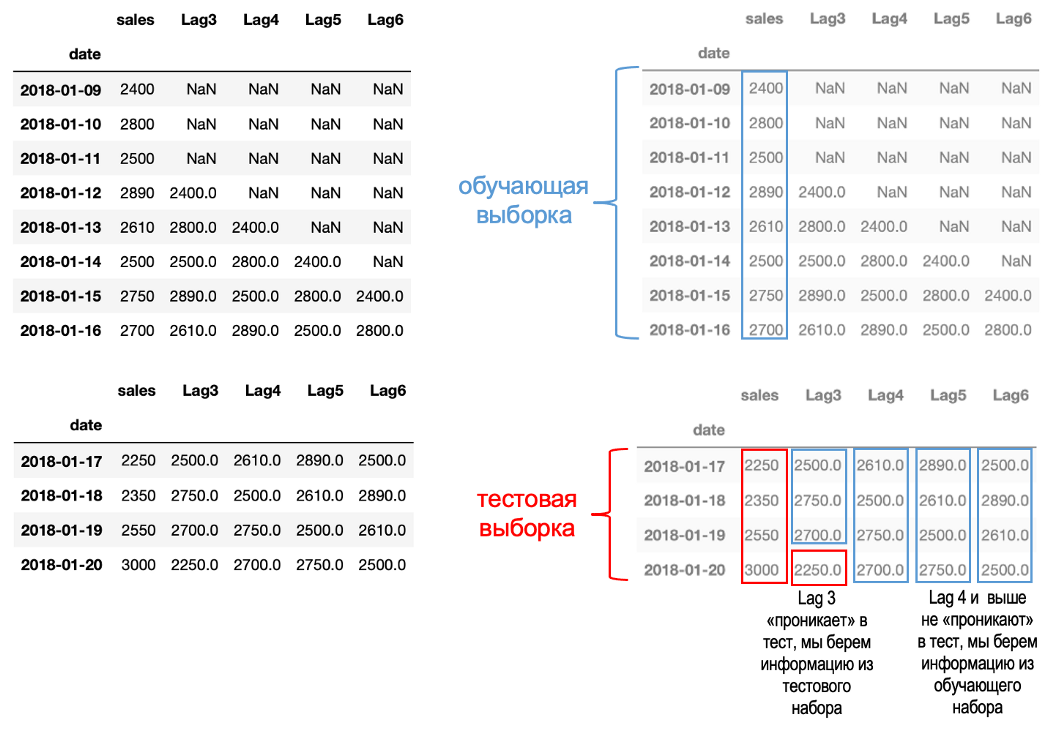
\includegraphics[scale=0.4]{figures/lags.png}
	\caption{ Лаги, у которых порядок равен горизонту прогнозирования или превышает его, не используют тестовую выборку }\label{fig:lags}
\end{figure}



Теперь создадим лаги, скользящее среднее, скользящее среднее абсолютное отклонение, обучим модель \texttt{LGBMModelMultiSegment}, получим прогнозы и визуализируем их
\begin{lstlisting}[
style = ironpython,
numbers = none,
]
# создаем экземпляр класса LagTransform для генерации лагов,
# с помощью in_column задаем переменную, на основе которой
# генерируем лаги, мы будем генерировать лаги порядка от 8 до 23, 
# порядок лагов не должен быть меньше длины горизонта
lags = LagTransform(in_column='target', 
				lags=list(range(8, 24, 1)), 
				out_column='lag')
# создаем экземпляр класса MeanTransform для вычисления 
# скользящего среднего по заданному окну
mean8 = MeanTransform(in_column='target', 
				window=8, 
				out_column='mean8')
# создаем экземпляр класса MadTransform для вычисления 
# среднего абсолютного отклонения по заданному окну
mad8 = MadTransform(in_column='target',
				window=8, 
				out_column='mad8')
# добавляем лаги, mean8, mad8 в обучающую выборку
train_ts.fit_transform([lags, mean8, mad8])
# создаем экземпляр класса LGBMModelPerSegment
model = LGBMModelPerSegment()
# обучаем модель
model.fit(train_ts)
# формируем тестовый набор
future_ts = train_ts.make_future(HORIZON)
# получаем прогнозы
forecast_ts = model.forecast(future_ts)
# оцениваем качество прогнозов
smape(y_true=test_ts, y_pred=forecast_ts)
\end{lstlisting}

\subsection{Работа с несколькими временными рядами}

Прогнозирование нескольких временных рядов. Загрузим набор, в котором каждому сегменту соответствует свой временной ряд
\begin{lstlisting}[
style = ironpython,
numbers = none	
]
original_df = pd.read_csv("data.csv")
original_df.head()

df = TSDataset.to_dataset(original_df)
\end{lstlisting}

Вновь воспользуемся моделью CatBoost с помощью класса CatBoostModelMultiSegment. Перед построением модели выполним некоторые преобразования и создадим новые признаки для наших рядов.

Нам понадобятся следующие классы-трансформеры:
\begin{itemize}
	\item класс \texttt{LogTransform} для логарифмирования и экспонецирования перерменной (логарифмирование позволяет сгладить негативное влияние выборосов объективной природы, помогает выделить тренд),
	
	\item \texttt{LinearTrendTransform} для прогнозирования тренда, удаления тренда из данных и добавления тренда к прогнозам (это необходимо для деревьев решений и для ансамблей деревьев решений, \underline{\emph{не умещющих экстраполировать}}),
	
	\item \texttt{LagTransform} для генерации лагов,
	
	\item \texttt{DateFlagsTransform} для генерации признаков на основе дат -- порядковый номер дня недели, порядковый номер дня месяца, порядковый номер недели в месяце и пр.,
	
	\item \texttt{MeanTransform} для вычисления скользящего среднего по заданному окну.
\end{itemize}

Сначала выполним логарифмирование зависимой переменной, а затем вычтем из нее тренд. Потом на основе пролагрифмированной зависимой переменной с удаленным трендом мы создадим лаги и скользящие средние, добавим календарные признаки.

\begin{lstlisting}[
style = ironpython,
numbers = none
]
# создаем экземпляр класса LogTransform для логарифмирования 
# и экспоненцирования зависимой переменной
log = LogTransform(in_column='target')

# создаем экземпляр класса LinearTrendTransform 
# для прогнозирования тренда, удаления тренда из 
# данных и добавления тренда к прогнозам
trend = LinearTrendTransform(in_column='target')

# создаем экземпляр класса SegmentEncoderTransform 
# для кодирования меток сегментов целочисленными 
# значениями в лексикографическом порядке (LabelEncoding): 
# сегменты a, b, c, d получат значения 0, 1, 2, 3
seg = SegmentEncoderTransform()

# создаем экземпляр класса LagTransform 
# для генерации лагов (c лага 31 по лаг 95)
lags = LagTransform(in_column='target', 
	lags=list(range(31, 96, 1)), 
	out_column='lag')
	
# создаем экземпляр класса DateFlagsTransform для 
# генерации признаков на основе дат - порядковый 
# номер дня недели, порядковый номер дня месяца,
# порядковый номер недели в месяце, порядковый 
# номер недели в году, порядковый номер месяца 
# в году, индикатор выходных дней
d_flags = DateFlagsTransform(day_number_in_week=True,
	day_number_in_month=True,
	week_number_in_month=True,
	week_number_in_year=True,
	month_number_in_year=True,
	special_days_in_week=[5, 6], 
	out_column='datetime')
	
# создаем экземпляр класса MeanTransform для вычисления 
# скользящего среднего по заданному окну
mean30 = MeanTransform(in_column='target', 
	window=30, 
	out_column='mean30')
\end{lstlisting}

Разбиваем набор (наш объект TSDataset) на обучающую и тестовую выборки с учетом временной структуры. Здесь горизонт прогнозирования сосавит 31 день
\begin{lstlisting}[
style = ironpython,
numbers = none
]
# разбиваем набор на обучающую и тестовую выборки 
# с учетом временной структуры
train_ts, test_ts = ts.train_test_split(
    train_start="2019-01-01",
    train_end="2019-11-30",
    test_start="2019-12-01",
    test_end="2019-12-31",
)

# выполняем преобразования набора
train_ts.fit_transform([
	log,  # логарифмируем
	trend,  # удаляем тренд
	lags,  # вычисляем лаги
	d_flags,  # вычисляем признаки на основе дат
	seg,  # кодируем метки сегментов
	mean30  # вычисляем скользящее среднее
])
\end{lstlisting}

Задаем явно горизонт в 31 день, обучаем модель CatBoost, оцениваем качество прогнозов и визуализируем прогнозы. Кроме того, не забываем выполнить обратные преобразования (добавление тренда, экспонецирование зависимой переменной) с помощью метода \texttt{.inverse\_transform()} для обучающего набора для правильной визуализации значений зависимой переменной в обучающей выборке.

\begin{lstlisting}[
style = ironpython,
numbers = none
]
# задаем горизонт прогнозирования
HORIZON = 31
# создаем экземпляр класса CatBoostModelMultiSegment
model = CatBoostModelMultiSegment()
# обучаем модель CatBoost
model.fit(train_ts)
# формируем набор, для которого нужно получить прогнозы,
# длина набора определяется горизонтом прогнозирования
future_ts = train_ts.make_future(HORIZON)

# получаем прогнозы
forecast_ts = model.forecast(future_ts)

# оцениваем качество прогнозов
smape(y_true=test_ts, y_pred=forecast_ts)
\end{lstlisting}

Выполняем обратное преобразование для обратной выборки (добавляем тренд, делаем экспоненцирование переменной \texttt{target})
\begin{lstlisting}[
style = ironpython,
numbers = none
]
train_ts.inverse_transform()
plot_forecast(forecast_ts, test_ts, train_ts, n_train_sample=20)
\end{lstlisting}

Для более надежной оценки качества модели \texttt{CatBoost} воспользуемся \emph{перекрестной проверкой расширяющимся окном}
\begin{lstlisting}[
style = ironpython,
numbers = none
]
pipe = Pipeline(
    model=model,
    transform=[
        log,
        trend,
        seg,
        lags,
        d_flags,
        mean30,
    ],
    horizon=HORIZON,
)
metrics, forecast, info = pipe.backtest(ts, [smape], aggregate_metrics=True)
\end{lstlisting}

Ансамбль бустингов
\begin{lstlisting}[
style = ironpython,
numbers = none,
]
transforms = [log, trend, seg, lags, d_flags, mean30]
catboost_pipeline = Pipeline(
    model=CatBoostModelMultiSegment(),
    transforms=transforms,
    horizon=HORIZON
)

lightgbm_pipeline = Pipeline(
    model=LGBMModelMultiSegment(),
    transforms=transforms,
    horizon=HORIZON
)

xgboost_pipeline = Pipeline(
    model=XGBModelMultiSegment(learning_rate=0.2, n_estimators=500, max_depth=1),
    transforms=transforms,
    horizon=HORIZON
)

pipeline_names = ["catboost", "lightgbm", "xgboost"]
pipelines = [catboost_pipeline, lightgbm_pipeline, xgboost_pipeline]

voting_ensemble = VotingEnsemble(
    pipelines=pipelines,
    weight=[1, 1, 2],
    n_jobs=1
)

metrics, forecast, _ = voting_ensemble.backtest(
    ts=ts, metrics=[SMAPE()], n_folds=3, aggregate_metrics=True, n_jobs=1
)
\end{lstlisting}

Заметим, что скользящее среднее используется не только для конструирования признаков, но и в качестве прогнозной модели (когда прогноз -- скользящее среднее $ n $ последних наблюдений), а также для сглаживания выборосов, краткосрочных колебаний и более четкого выделения долгосрочных тенденций в ряде данных.

\section{Генерация признаков и кодирование категориальных признаков}

Процесс создания признакового пространства зависит от модели, которую будем использовать:
\begin{itemize}
	\item OHE-кодирование предпочтительнее для линейных моделей,
	
	\item умное кодирование категорий -- для деревьев,
	
	\item выбросы можно не удалять для робастной модели.
\end{itemize}

Если в тестовом наборе данных присутствуют категории, которых не было в обучающем наборе данных, то нужно принять решение о том, как их кодировать. Например, категорию из нового набора данных можно отнести к самомой опасной категории из тех, категорий, которые присутствуют в обучающем наборе данных.

Еще категории можно кодировать по разным признакам.

Можно кодировать признаки по мощности (Count Encoding): сколько раз каждая уникальная категория встречалась в категориальном признаке. Проблема в том, что некоторые категории могут встречаться одинаковое количество раз (коллизия). Чтобы различать такие категории можно добавить шум, т.е. $ count + \varepsilon $. Мелкие и новые категории объединяют в одну.

Кодирование по мощности можно использовать, если требуется быстро решить задачу.

\subsection{Кодирование одного категориального признака по другому категориальному признаку с помощью сингулярного разложения}

Если матрица признакового описания объекта состоит только из категориальных признаков, то можно кодировать один признак на основе другого
\begin{lstlisting}[
style = ironpython,
numbers = none
]
from numpy.linalg import svd

def code_factor(data, cat_feature, cat_feature2):
    """
    Кодирование признака на основе другого признака
    """
    ct = pd.crosstab(data[cat_feature], data[cat_feature2])
    u, _, _ = svd(ct.values)
    coder = dict(zip(ct.index, u[:, 0]))  # берем только первый сингулярный вектор
    
    return data[cat_feature].map(coder)
\end{lstlisting}

Сингулярное разложение (Singular Value Decomposition, SVD) -- декомпозиция вещественной матрицы с целью ее приведения к каноническому виду. Сингулярное разложение является удобным методом при работе с матрицами. Оно показывает геометрическую структуру матрицы и позволяет наглядно представить имеющиеся данные. В числе прочего SVD позволяет вычислять обратные и псевдообратные матрицы большого размера, что делает его полезным инструментом при решении задач регрессионного анализа.

\remark{
В числе прочего с помощью сингулярного разложения можно решать задачи обращения или пвседообращения матриц большого размера
}

Для любой вещественной $ (n \times n) $-матрицы $ A $ существуют две вещественные ортогональные $ (n \times n) $-матрицы $ U $ и $ V $ такие, что
\begin{align*}
	\Lambda = U^{T} A V,
\end{align*}
где $ \Lambda $ -- диагональная матрица.

Матрицы $ U $ и $ V $ выбираются так, чтобы диагональные элементы матрицы $ A $ имели вид
\begin{align*}
	\lambda_1 \geqslant \lambda_2 \geqslant \ldots \geqslant \lambda_r > \lambda_{r + 1} = \lambda_n = 0,
\end{align*}
где $ r $ -- ранг матрицы $ A $.

В частности, если $ A $ невырождена (то есть существует обратная матрица $ A^{-1}, \det A \neq 0 $), то
\begin{align*}
	\lambda_1 \geqslant \lambda_2 \geqslant \ldots \geqslant \lambda_n > 0.
\end{align*}

\underline{Столбцы} матриц $ U $ и $ V $ называются соответсвенно \emph{левыми} и \emph{правыми сингулярными векторами}, а значения диагонали матрицы $ \Lambda $ -- \emph{сингулярными числами}.

Эквивалентная запись сингулярного разложения
\begin{align*}
	A = U \Lambda V^{T}
\end{align*}

Например, матрица
\begin{align*}
	A = \begin{pmatrix}
		0.96 & 1.72 \\
		2.28 & 0.96
	\end{pmatrix}
\end{align*}
имеет сингулярное разложение
\begin{align*}
	A = U \Lambda V^{T} =
	\begin{pmatrix}
		0.6 & 0.8\\
		0.8 & -0.6
	\end{pmatrix}
    \begin{pmatrix}
    	3 & 0\\
    	0 & 1
    \end{pmatrix}
    \begin{pmatrix}
    	0.8 & -0.6 \\
    	0.6 & 0.8
    \end{pmatrix}^T
\end{align*}

Легко увидеть, что матрицы $ U $ и $ V $ ортогональны,
\begin{align*}
	U^T U = UU^T = I, \quad V^T V = V V^T = I,
\end{align*}
и сумма квадратов значений их столбцов равна единице.

Для \emph{прямоугольных} матриц существует так называемое экономное представление сигнулярного разложения
\begin{align*}
	A_{(m \times n)} = U_{(m \times r)} \Lambda_{(r \times r)} V_{(r \times n)}^T,
\end{align*}
где $ r = \min(m, n) $.

\noindent\emph{Сингулярное разложение и собственные числа матрицы}

Сингулярное разложение обладает свойством, которое связывает задачу отыскания сингулярного разложения и задачу отыскания собственных векторов. Собственный вектор $ x $ матрицы $ A $ -- такой вектор, при котором выполняется условие $ A x = \lambda x $, где $ \lambda $ -- собственное число.

Так как матрицы $ U $ и $ V $ ортогональные, то
\begin{align*}
	A A^T = U \Lambda \underbrace{V^T V}_{= I} \Lambda U^T = U \Lambda^2 U^T,\\
	A^T A = V \Lambda \underbrace{U^T U}_{= I} \Lambda V^T = V \Lambda^2 V^T.
\end{align*}

Умножая оба выражения справа соответсвенно на $ U $ и $ V $, получаем
\begin{align*}
	A A^T U = U \Lambda^2,\\
	A^T A V = V\Lambda^2.
\end{align*}

Из этого следует, что \underline{столбцы} матрицы $ U $ являются собственными векторами матрицы $ AA^T $, а квадраты сингулярных чисел $ \Lambda = \text{diag}(\lambda_1, \ldots, \lambda_r) $ -- ее собственным числам. Также \underline{столбцы} матрицы $ V $ являются собственными векторами матрицы $ A A^T $, а квадраты сингулярных чисел являются ее собвственными числами.

\noindent\emph{SVD и норма матриц}

Евклидова норма
\begin{align*}
	|A|_E = \max\limits_{|x| = 1} \dfrac{ |A x| }{ |x| }.
\end{align*}

Норма Фробениуса
\begin{align*}
	|A|_F = \sqrt{\sum_{i=1}^{m}\sum_{j=1}^{n} a_{ij}^2}.
\end{align*}

Если известно сингулярное разложение, то обе эти нормы легко вычислить. Пусть $ \lambda_1, \ldots, \lambda_r $ -- сингулярные числа матрцы $ A $, отличные от нуля.

Тогда $ |A|_E = \lambda_1 $ и $ |A|_F = \sqrt{\sum\limits_{k=1}^{r} \lambda_k^2} $.

\noindent\emph{Нахождение псевдообратной матрицы с помощью SVD}

Если $ (m \times n) $-матрица $ A $ является \emph{вырожденной} или \emph{прямоугольной}, то обратной матрицы $ A^{-1} $ для нее \underline{не существует}. 

Однако, для $ A $ может быть найдена псевдообратная матрица $ A^{+} $ -- такая матрица, для которой выполняются условия
\begin{align*}
	A^{+}A &= I_n,\\
	A A^{+} &= I_m,\\
	A^{+} A A^{+} &= A^{+},\\
	A A^{+} A &= A.
\end{align*}

Пусть найдено разложение матрицы $ A $ вида
\begin{align*}
	A = U \Lambda V^T,
\end{align*}
где $ \Lambda = \text{diag}(\lambda_1, \ldots, \lambda_r), r=\min(m, n) $ и $ U^T U = I_m, VV^T = I_n $.

Тогда матрица
\begin{align*}
	A^+ = V^T \Lambda^{-1}U
\end{align*}
является для матрицы $ A $ \emph{псевдообратной}.

\noindent\emph{Усеченное SVD при обращении матриц}

Для получения обращения, устойчивого к малым изменениям значений матрицы $ A $, используется усеченное SVD. Пусть матрица $ A $ представлена в виде $ A = U\Lambda V^T $.

Тогда \emph{усеченная псевдообратная матрица} $ A_s^+ $
\begin{align*}
	A_s^+ = V \Lambda_s^{-1} U^T,
\end{align*}
где $ \Lambda_s^{-1} = \text{diag}(\lambda_1^{-1}, \ldots, \lambda_s^{-1}, 0, \ldots, 0) $ -- $ (n \times n) $-диагональная матрица, $ s $ -- первые $ s $ сингулярных чисел, $ s \leqslant \text{rang} A $.

Есть еще хэш-кодирование (\texttt{sklearn.feature\_extractoin.FeatureHasher}). Для быстрого анализа пойдет, но применяется редко.

Можно кодировать категории по целевой переменной (Target Encoding). Есть варианты целевого кодирования по среднему (Mean Target Encoding), по стандартному отклонению (Std Target Enconing) и т.д. Подход для \emph{любого} алгоритма. Кодирование по значению целевой переменной <<логично>>.

Главная проблема: неадекватная кодировка мелких категорий + слияние этих категорий. Нельзя допустить утечки значений целевой переменой!

Теоретически можно кодировать категориальные признаки на обучающем поднаборе, а обучать алгоритм на отложенной выборке, но это не очень здорово, так как теряем значительную часть данных на этапе кодирования.

Кодирование по \emph{предыдущим} объектам (CatBoost). Одна категория в обучении кодируется по-разному, а на контроле фиксировано
\begin{lstlisting}[
style = ironpython,
numbers = none	
]
gb = data.groupby(name)
data[name + "_cb"] = (gb["target"].cumsum() - data["target"]) / gb.cumcount()
\end{lstlisting}

Получаются более менее адекватные значения, но без подглядывания. В самом начале кодирования (в первых строках) пока статистика не наберется значения будут неадекватные. Можно тасовать матрицу признакового описания объекта, а затем усреднять результаты кодировки.

На практике хорошо работает смесь подходов!


\section{Перестановочная важность признаков и важность признаков по Шепли}

Полезный ресурс \url{https://scikit-learn.org/stable/modules/permutation_importance.html}

Статья Дьяконова \href{https://dyakonov.org/2018/08/28/%d0%b8%d0%bd%d1%82%d0%b5%d1%80%d0%bf%d1%80%d0%b5%d1%82%d0%b0%d1%86%d0%b8%d0%b8-%d1%87%d1%91%d1%80%d0%bd%d1%8b%d1%85-%d1%8f%d1%89%d0%b8%d0%ba%d0%be%d0%b2/}{про интерпретацию черных ящиков}

Важность признаков -- числовые оценки, насколько каждый признак \emph{важен} для решения поставленной задачи.

{\color{red} Плохой метод -- чем чаще выбирался признак, тем лучше.} Дело в том, что признак может действительно часто выбираться, но на более низких уровнях дерева (дальше от корня). Другими словами, признак выбирается часто, но используется для построения небольших <<уточняющих>> разбиений (\pic{fig:feature_imp}). Как правило, все наоборот. Если признак выбирается часто, значит модель не может по каким-то причинам сразу получить от него нужную информацию.

\begin{figure}[h]
	\centering
	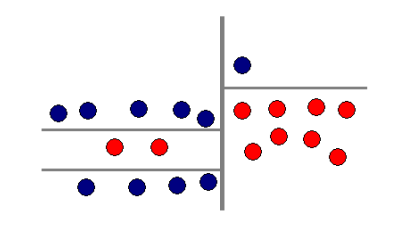
\includegraphics[scale=1.]{figures/feature_imp.png}
	\caption{ К вопросу о важности признака по частоте его выбора. Признак по оси $ x $ выбирается только один раз, а признак по оси $ y $ выбирается три раза, но очевидно, что первый признак лучше справляется с задачей }\label{fig:feature_imp}
\end{figure}

{\color{red}Нельзя отбрасывать признаки по порогу.}

Перестановочная важность признаков и важность признаков по Шепли обладают свойством \emph{согласованности} (если модель изменить так, что она более существенно начинает зависеть от какого-то признака, то его важность не убывает).

Подход вычисления \textbf{\itshape перестановочной важности признаков} (Permutation Feature Importance):
\begin{itemize}
	\item (+) не меняет распределение по конкретному признаку (так как рассматриваемый признак просто перемешивается),
	
	\item (+) не требует обучать модель заново -- обученную модель тестируют на отложенной выборке с испорченным признаком,
	
	\item (+) можно применять на любых алгоритмах,
	
	\item (+) самый надежный метод,
	
	\item (+) в бутсрепе можно использовать OOB-контроль (строить дерево и на зкземплярах, не попавших в дерево, вычислять перестрановочную важность),
	
	\item (-) очень медленный.
\end{itemize}

\remark{
Вместо метрик качества для вычисления перестановочной важности можно использовать что-то другое. Например, долю верно классифицирующих деревьев
}

Идея перестановочной важности признаков: признак важный, если его перетасовка снижает качество. Можно вычислять перестановочную важность признаков на \emph{обучающем поднаборе данных} (вроде как бы можно, но лучше использовать отложенную выборку PFI-holdout), на \emph{отложенном контроле} (тестовый поднабор данных PFI-holdout, \pic{fig:PFI-holdout}) и на любой схеме \emph{валидации} (надежнее использовать валидацию). 

\begin{figure}[h]
	\centering
	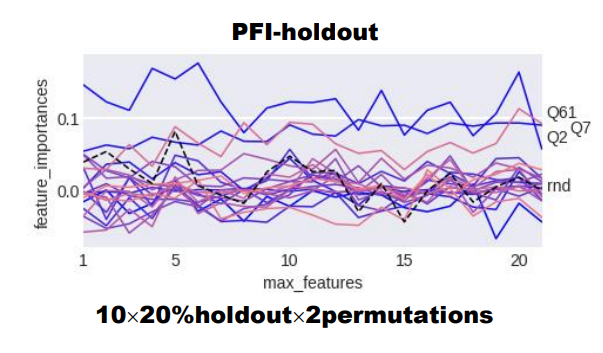
\includegraphics[scale=1.]{figures/PFI-holdout.png}
	\caption{ Перестановочная важность признаков, вычисленная на отложенной выборке }\label{fig:PFI-holdout}
\end{figure}

Перестановочная важность скоррелиррованных признаков может размазываться между ними.

Можно удалять признаки (Drop-column importance), но тогда каждый раз нужно будет заново обучать модель. Однако при этом результат более однозначный. Используется редко!

Если два признак коррелируют друг с другом, то перестановка одного из них не будет значимо сказываться на эффективности модели, потому что она может извлечь требуемую информацию из второго коррелирующего признака. Одним из способов работы с мультиколлинеарными признаками является иерархическая кластеризация на базе ранговых корреляций Спирмена, выбор порога отсечения и сохранение одного признака из каждого кластера.

\remark{
Важности признаков, полученные с помощью \texttt{feature\_importances\_} (важность по неоднородности), встроенного в алгоритмы построения ансамблей деревьев -- это НЕ важности признаков для решения задачи, а лишь для настройки конкретной модели. Этот подход не обладает свойством согласованности!!!}

В разделе 4.2.2 Relation to impurity-based importance in trees документации sklearn говорится, что impurity-based importance (\emph{важность признаков по неоднородности}; еще называют Gini importance) сильно смещена и отдает предпочтение \underline{высококардинальным} признакам (обычно вещественным) по сравнению с низкокардинальными признаками, такими как бинарные или категориальные признаки с небольшим числом категорий. Кроме того, важность по неоднородности годится только для деревьев и их ансамблей.

\textbf{\emph{Важность по Шепли}} $ i $-ого признака вычисляется следующим образом
\begin{align*}
	\varphi_i = \sum_{S \subseteq \{1, 2, \ldots, n\} \setminus \{i\}} \dfrac{ | S |! (n - |S| - 1)! }{ n! } \big( f(S \cup \{i\}) - f(S) \big),
\end{align*}
где $ f(S) $ -- ответ модели, обученной на подмножестве $ S $ множества $ n $ признаков (на конкретном объекте -- вся формула записывается для конкретного объекта).

Вычисление требует переобучения модели на всевозможных подмножествах признаков, поэтому на практике применяются приближения формулы, например, с помощью метода Монте-Карло.

Замечания по методам оценки важности признаков:
\begin{itemize}
	\item \underline{\itshape нет идеального алгоритма оценки важности признаков} (для любого можно подобрать пример, когда он плохо работает),
	
	\item если много похожих признаков (например, сильно коррелированных), то важность может <<делиться между ними>>, поэтому не рекомендуется отбрасывать признаки по порогу важности,
	
	\item есть старая рекомендация (впрочем, без теоретического обоснования): модель для решения задачи и оценки важности должны основываться на разных парадигмах (например, оценивать важность с помощью случайного леса и потом настраивать его же на важных признаках не рекомендуется). {\color{blue}То есть не рекомендуется оценивать важность и решать ML-задачу одним и тем же алгоритмом!!!}
\end{itemize}

Советы Дьяконова:
\begin{itemize}
	\item можно выбрать некоторое подмножество признаков и потом то добавить $ k $ признаков, то отнять $ l $,
	
	\item оценивать важность не обязательно с помощью лучшей модели (то есть не нужно строить супермодель для того, чтобы оценить важность признаков!)
	
	\item перестановочная важность самая естественная (но есть нюансы: коррелированность признаков, стабильность оценки и т.п.),
	
	\item есть и другие подходы и удобные библиотеки (SHAP, например).
\end{itemize}



\section{Приемы работы с библиотекой Catboost}

Онлайн документация пакета \url{https://catboost.ai/en/docs/concepts/python-reference_catboostregressor}.

\subsection{Установка CatBoost}

Установить пакет можно с помощью менеджера \texttt{conda} (или с помощью \texttt{pip})
\begin{lstlisting}[
style = bash,
numbers = none
]
$ conda config --show channels
# если канала conda-forge нет в списке, то следует его добавить 
$ conda config --add channels conda-forge
$ conda install catboost
$ pip install catboost
\end{lstlisting}

\subsection{Ключевые особенности пакета}

\subsection{Параметры}

\remark{
Помимо \texttt{iterations} и \texttt{learning\_rate} у CatBoost 5 важнейших гиперпараметров: \texttt{max\_depth}, \texttt{l2\_leaf\_reg}, \texttt{border\_count}, \texttt{random\_strength} и \texttt{bagging\_temperature}
}

Применительно к \texttt{random\_strength} замечено, что часто значение, близкое к 0 (примерно, 0.15), дает лучшее качество. Если переменных много, можно попробовать настраивать \texttt{rsm}.

В случае дисбаланса классов будет полезным настраивать
\begin{itemize}
	\item либо гиперпараметр \texttt{auto\_class\_weights},
	
	\item либо гиперпараметры \texttt{class\_weights} и \texttt{scale\_pos\_weight}
\end{itemize}
при этом не нужно настраивать эти параметры одновременно.

Можно сначала при \emph{небольшом} числе итераций найти оптимальные значения гиперпараметров, \emph{меньше} всего зависящие от количества итераций (речь прежде всего идет об \texttt{auto\_class\_weights}, \texttt{max\_depth}; при этом \texttt{learning\_rate} и \texttt{rsm} зависят от количества итераций, поэтому нам для небольшого количества итераций придется увеличить темп обучения, а варьирование \texttt{rsm} сделать минимальным). Затем можно построить модель с найденными оптимальными значениями гиперпараметров  \texttt{auto\_class\_weights}, \texttt{max\_depth} и \texttt{rsm}, но уже с большим количеством деревьев, при этом, разумеется помня о двух вещах:
\begin{itemize}
	\item при большом количестве итераций нужно уменьшить темп обучения,
	
	\item выбирая меньшее значение \texttt{rsm}, нужно задавать больше итераций.
\end{itemize}

Ознакомится с описанием параметров можно здесь \url{https://catboost.ai/en/docs/references/training-parameters/}

Общие параметры:
\begin{itemize}
	\item \verb|loss_function| (objective) -- функция потерь, которая используется на шаге обучения модели.
	
	\item \texttt{iterations} -- максимальное число деревьев в ансамбле,
	
	\item \verb*|learning_rate| -- темп обучения,
	
	\item \verb*|l2_leaf_reg| -- коэффициент при члене $ L_2 $-регуляризации,
	
	\item \verb*|bagging_temperature| -- задает настройки Байесовского бутстрапа
\end{itemize}



\subsection{Классификатор CatBoostClassfier}

Класс \texttt{CatBoostClassifier}

\begin{lstlisting}[
style = ironpython,
numbers = none	
]
class CatBoostClassifier(
		iterations=None,
		learning_rate=None,
		depth=None,
		l2_leaf_reg=None,
		model_size_reg=None,
		rsm=None,
		loss_function=None,
		border_count=None,
		feature_border_type=None,
		per_float_feature_quantization=None,                         
		input_borders=None,
		output_borders=None,
		fold_permutation_block=None,
		od_pval=None,
		od_wait=None,
		od_type=None,
		nan_mode=None,
		counter_calc_method=None,
		leaf_estimation_iterations=None,
		leaf_estimation_method=None,
		thread_count=None,
		random_seed=None,
		use_best_model=None,
		verbose=None,
		logging_level=None,
		metric_period=None,
		ctr_leaf_count_limit=None,
		store_all_simple_ctr=None,
		max_ctr_complexity=None,
		has_time=None,
		allow_const_label=None,
		classes_count=None,
		class_weights=None,
		one_hot_max_size=None,
		random_strength=None,
		name=None,
		ignored_features=None,
		train_dir=None,
		custom_loss=None,
		custom_metric=None,
		eval_metric=None,
		bagging_temperature=None,
		save_snapshot=None,
		snapshot_file=None,
		snapshot_interval=None,
		fold_len_multiplier=None,
		used_ram_limit=None,
		gpu_ram_part=None,
		allow_writing_files=None,
		final_ctr_computation_mode=None,
		approx_on_full_history=None,
		boosting_type=None,
		simple_ctr=None,
		combinations_ctr=None,
		per_feature_ctr=None,
		task_type=None,
		device_config=None,
		devices=None,
		bootstrap_type=None,
		subsample=None,
		sampling_unit=None,
		dev_score_calc_obj_block_size=None,
		max_depth=None,
		n_estimators=None,
		num_boost_round=None,
		num_trees=None,
		colsample_bylevel=None,
		random_state=None,
		reg_lambda=None,
		objective=None,
		eta=None,
		max_bin=None,
		scale_pos_weight=None,
		gpu_cat_features_storage=None,
		data_partition=None
		metadata=None,
		early_stopping_rounds=None,
		cat_features=None,
		grow_policy=None,
		min_data_in_leaf=None,
		min_child_samples=None,
		max_leaves=None,
		num_leaves=None,
		score_function=None,
		leaf_estimation_backtracking=None,
		ctr_history_unit=None,
		monotone_constraints=None,
		feature_weights=None,
		penalties_coefficient=None,
		first_feature_use_penalties=None,
		model_shrink_rate=None,
		model_shrink_mode=None,
		langevin=None,
		diffusion_temperature=None,
		posterior_sampling=None,
		boost_from_average=None,
		text_features=None,
		tokenizers=None,
		dictionaries=None,
		feature_calcers=None,
		text_processing=None
)
\end{lstlisting}

LogLoss применяется для задач бинарной классификации (когда целевей вектор содиржит только два уникальных значения или когда параметр \verb|target_border is not None|).

MultiClass используется в задачах мультиклассовой классификации (когда целевой вектор содержит более 2 уникальных значений или параметр \verb|border_count is None|)

\subsection{Регрессор CatBoostRegressor}

Помимо \texttt{iterations} и \texttt{learning\_rate} у CatBoost 5 важнейших гиперпараметров:
\begin{itemize}
	\item \texttt{max\_depth}: мак,
	
	\item \texttt{l2\_leaf\_reg},
	
	\item \texttt{border\_count},
	
	\item \texttt{random\_strength},
	
	\item \texttt{bagging\_temperature}.
\end{itemize}

\subsection{Функции потерь и метрики качества}

\subsubsection{Для классификации}

Для мультиклассификации \url{https://catboost.ai/en/docs/concepts/loss-functions-multiclassification}

\emph{Функции потерь}
\begin{itemize}
	\item LogLoss
\begin{align*}
	- \dfrac{ \sum\limits_{i=1}^N w_i \big( c_i \log p_i + (1 - c_i) \log (1 - p_i) \big) }{ \sum\limits_{i=1}^{N} w_i },
\end{align*}

    \item CrossEntropy
\begin{align*}
	- \dfrac{ \sum\limits_{i=1}^N w_i \big( t_i \log p_i + (1 - t_i) \log (1 - p_i) \big) }{ \sum\limits_{i=1}^{N} w_i },
\end{align*}
\end{itemize}

\emph{Метрики качества}
\begin{itemize}
	\item Precision (точность),
	
	\item Recall (полнота),
	
	\item F1 (гармоническое среднее),
	
	\item BalancedAccuracy
\begin{align*}
	\dfrac{1}{2} \Big( \dfrac{TP}{T} + \dfrac{TN}{N} \Big),
\end{align*}

    \item BalancedErrorRate
\begin{align*}
	\dfrac{1}{2} \Big( \dfrac{FP}{TN + FP} + \dfrac{FN}{FN + TP} \Big),
\end{align*}

    \item AUC,
    
    \item BrierScore,
    
    \item HingeLoss,
    
    \item HammingLoss
\begin{align*}
	\dfrac{ \sum\limits_{i=1}^{N} w_i [[p_i > 0.5] == t_i] }{ \sum\limits_{i=1}^{N} w_i},
\end{align*}

    \item Kappa
\begin{align*}
	1 - \dfrac{1 - Accuracy}{1 - RAccuracy},\\
	RAccuracy = \dfrac{ (TN + FP) (TN + FN) + (FN + TP)(FP + TP) }{ \Big( \sum\limits_{i=1}^{N} w_i \Big)^2 }
\end{align*}

    \item LogLikelihoodOfPrediction.
\end{itemize}

\subsubsection{Для регрессии}

\emph{Метрики качества, которые могут играть роль функции потерь}

\begin{itemize}
	\item MultiRMSE (в случае мультирегрессии)
\begin{align*}
	\Biggl( \dfrac{ \sum\limits_{i=1}^N \sum\limits_{d=1}^{dim} (a_{i,d} - t_{i,d})^2 w_i }{ \sum\limits_{i=1}^N w_i } \Biggr)^{1/2}
\end{align*}
	
	\item MAE
\begin{align*}
	\dfrac{ \sum\limits_{i=1}^{N} w_i | a_i - t_i |}{ \sum\limits_{i=1}^{N} w_i },
\end{align*}

    \item MAPE
\begin{align*}
	\dfrac{ \sum\limits_{i=1}^{N} w_i \dfrac{ | a_i - t_i | }{ \max (1, | t_i |) } }{ \sum\limits_{i=1}^N w_i }
\end{align*}

    \item Poisson
\begin{align*}
	\dfrac{ \sum\limits_{i=1}^N w_i (e^{ a_i } - a_i t_i) }{ \sum\limits_{i=1}^N w_i },
\end{align*}

   \item Quantile (большие значения $ \alpha $ сильнее штрафуют за заниженные прогнозы)
\begin{align*}
	\dfrac{ \sum\limits_{i=1}^N \Big( \alpha - 1[t_i \leqslant a_i] \Big) (t_i - a_i) w_i}{ \sum\limits_{i=1}^N w_i },
\end{align*}

    \item RMSE
\begin{align*}
	\Bigg( \dfrac{ \sum\limits_{i=1}^N (a_i - t_i)^2 w_i }{ \sum\limits_{i=1}^N w_i } \Bigg)^{1/2}
\end{align*}

    \item LogLinQuantile,
    
    \item Lq
\begin{align*}
	\dfrac{\sum\limits_{i=1}^N | a_i - t_i |^q w_i}{ \sum\limits_{i=1}^N w_i }
\end{align*}

    \item Huber
\begin{align*}
	L(t, a) = \sum_{i=0}^N l(t_i, a_i) \cdot w_i,\quad l(t, a) = 
	\begin{cases}
		\dfrac{1}{2} (t - a)^2, &| t - a | \leqslant \delta,\\
		\delta | t - a | - \dfrac{1}{2} \delta^2, &| t - a | > \delta.
	\end{cases}
\end{align*}

\item Excpectile
\begin{align*}
	\dfrac{ \sum\limits_{i=1}^N | \alpha - 1[t_i \leqslant a_i] | (t_i - a_i)^2 w_i }{ \sum\limits_{i=1}^N w_i }
\end{align*}

\item Tweedie
\begin{align*}
	\dfrac{ \sum\limits_{i=1}^N \Big( \dfrac{e^{a_i (2 - \lambda)}}{2 - \lambda} - t_i \dfrac{ e^{a_i ( 1 - \lambda)} }{ 1 - \lambda } \Big) w_i }{ \sum\limits_{i=1}^N w_i },
\end{align*}
где $ \lambda $ -- значение параметра дисперсии мощности,
\end{itemize}

\emph{Метрики качества}

\begin{itemize}
	\item SMAPE
\begin{align*}
	\dfrac{ 100 \sum\limits_{i=1}^N \dfrac{ w_i | a_i - t_i | }{ (|t_i| + |a_i|)/2 } }{ \sum\limits_{i=1}^N w_i }
\end{align*}

    \item R2 (коэффициент детерминации)
\begin{align*}
	1 - \dfrac{ \sum\limits_{i=1}^N w_i (a_i - t_i)^2 }{ \sum\limits_{i=1}^N w_i (\bar{t} - t_i)^2 }.
\end{align*}

    \item MSLE (среднеквадратическая логарифмическая ошибка)
\begin{align*}
	\dfrac{ \sum\limits_{i=1}^N w_i \big( \ln (1 + t_i) - \ln (1 + a_i) \big)^2 }{ \sum\limits_{i=1}^N w_i }
\end{align*}

    \item MedianAbsoluteError
\begin{align*}
	median(|t_1 - a_1|, \ldots, |t_N - a_N|)
\end{align*}
\end{itemize}

\section{Приемы работы с библиотеками Gym и Ecole}

\subsection{Gym}

Функция окружения (environment) \texttt{step} возвращает четыре значения:
\begin{itemize}
	\item \verb|observation| (object):  это объект, специфичный для окружающей среды и представляющий результат наблюдения за этой средой (например, состояние доски в настольной игре),
	
	\item \verb|reward| (float): вознаграждение, полученное за предыдущее действие. Масштаб варьируется в зависимости от среды, но цель всегда в том, чтобы сделать суммарное вознаграждение как можно больше,
	
	\item \verb|done| (boolean): флаг завершения эпизода. Многие (но не все) задачи разделены на четко определенные эпизоды, и \texttt{done = True} указывает на то, что эпизод завершился (например, мы потеряли последнюю жизнь в игре),
	
	\item \verb|info| (dict): диагонстическая информация, полезная для отладки.
\end{itemize}

Это просто реализация классического цикла <<агент -- среда>>. На каждом шаге агент совершает то или иное действие и среда возвращает наблюдения (observation) и вознаграждение (reward).

Процесс запускается вызовом функции \verb|reset()|, которая возвращает первое приближение \texttt{observation}.  
\begin{lstlisting}[
style=ironpython,
numbers=none
]
import gym
env = gym.make('CartPole-v0')
for i_episode in range(20):
    observation = env.reset()
    for t in range(100):
        env.render()
        print(observation)
        action = env.action_space.sample()
        observation, reward, done, info = env.step(action)
        if done:
            print("Episode finished after {} timesteps".format(t+1))
            break
env.close()
\end{lstlisting}

В этом примере мы отбирали случайные действия из пространства действий среды. Каждая среда поставляется с атрибутами \verb|action_space| и \verb|observation_space|. Эти атрибуты имеют тип \verb|Space| и описывают формат допустимых действий и наблюдений
\begin{lstlisting}[
style=ironpython,
numbers=none
]
import gym

env = gym.make("CartPole-v0")
print(env.action_space)  # Discrete(2)

print(env.observation_space)  # Box([-4.8000002e+00 -3.4028235e+38 -4.1887903e-01 -3.4028235e+38], [4.8000002e+00 3.4028235e+38 4.1887903e-01 3.4028235e+38], (4,), float32)
\end{lstlisting}

Пространство \texttt{Descrete} описывает фиксированный диапазон неотрицательных чисел, так что в данном случае допустимыми действиями будет 0 или 1. Пространство \texttt{Box} представляет $ n $-мерный ящик, так что в данном случае допустимыми наблюдениями будут 4-мерные массивы.

\subsection{Ecole}

Полезный ресурс о специальных приемах работы с задачами линейного программирования в частично-целочисленного постановке \url{https://www.gams.com/37/docs/UG_LanguageFeatures.html?search=sos1}

Полезный ресурс по математической оптимизации \url{https://scipbook.readthedocs.io/en/latest/}

\subsubsection{Observations}

Класс \texttt{ecole.observation.NodeBipartiteObs}: двудольный граф наблюдений для узлов branch-and-bound дерева. Оптимизационная задача представляется в виде гетерогенного двудольного графа. Между переменной и ограничением будет существовать ребро, если переменная присутствует в ограничении с ненулевым коэффициентом.

Метод \texttt{reset()} в Ecole принимает в качестве аргумента экземпляр проблемы. 

\section{Нейронные сети}

Теорема об универсальной аппроксимации (Hornik, 1991)

\emph{Любую} непрерывную функцию можно с любой точностью приблизить нейросетью глубины 2 с \emph{сигмоидной функцией активации} на скрытом слое и \emph{линейной функцией} на выходном слое.

Нейросеть глубины два с фиксированной функцией активации в первом слое и линейной функцией активации во втором слое может равномерно аппроксимировать (может быть при увеличении числа нейронов на первом слое) любую непрерывную функцию на компактном множестве тогда и только тогда, когда функция активации \emph{неполиномиальная}.

Что плохого в сигмоиде:
\begin{itemize}
	\item <<убивает>> градиенты,
	
	\item выходы не отцентрированы (легко устранить с помощьд $ \tanh $),
	
	\item вычисление экспоненты все-таки накладно
\end{itemize}

\remark{
Обратное распространение = SGD + дифференцирование сложных функций (\pic{fig:backprop})
}

\begin{figure}[h]
	\centering
	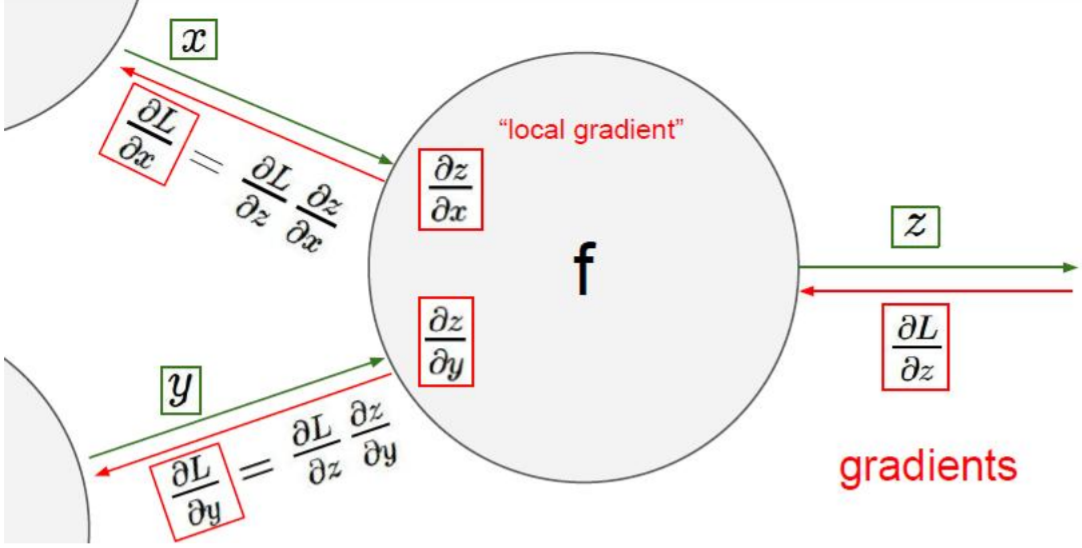
\includegraphics[scale=0.5]{figures/backprop.png}
	\caption{ Прямое распространение сигнала и обратное распространение градиента }\label{fig:backprop}
\end{figure}

\section{Борьба с переобучением в нейронных сетях}

\subsection{Нормировка}

Пусть даны признаки $ X = \{X_1, \ldots, X_m\} $.

Тогда

\emph{среднее признака}
\begin{align*}
	\mu = \dfrac{1}{m} \sum_{i=1}^m X_i,
\end{align*}

\emph{дисперсия признака}
\begin{align*}
	\sigma^2 = \dfrac{1}{m} \sum_{i=1}^m (X_i - \mu)^2
\end{align*}

\emph{нормировка}
\begin{align*}
	X = \dfrac{X - \mu}{\sqrt{\sigma^2}}
\end{align*}

\subsection{Инициализация весов}

Инициализация весов:
\begin{itemize}
	\item нарушить симметричность (чтобы нейроны были разные),
	
	\item недопустить насыщение нейрона (почти всегда близок к 0 или 1),
	
	\item ключевая идея -- входы на все слои должны иметь одинаковую дисперсию (для избегания <<насыщения>> нейронов).
\end{itemize}

Инициализация по Ксавье [Glorot \& Bengio, 2010]
\begin{align*}
	w_{ij}^{(k)} \sim U \Bigg[ - \sqrt{ \dfrac{ 6 }{ n_{in}^{(k)} + n_{out}^{(k)}} }, + \sqrt{ \dfrac{ 6 }{ n_{in}^{(k)} + n_{out}^{(k)}} } \, \Bigg].
\end{align*}

Дисперсия весов
\begin{align*}
	D[ w_{ij}^{(k)} ] = \dfrac{ 2 }{ n_{in}^{(k)} + n_{out}^{(k)} }.
\end{align*}

Формула выведена в предположении, что нет нелинейностей, т.е. $ z^{(k+1)} = f(W^{(k)} z^{(k)}) \equiv W^{(k)} z^{(k)} $.

Смотрим ошибку на отложенной выборке! Выбираем итерацию, на которой ошибка наименьшая (\pic{fig:lear_rate}).

\begin{figure}[h]
	\centering
	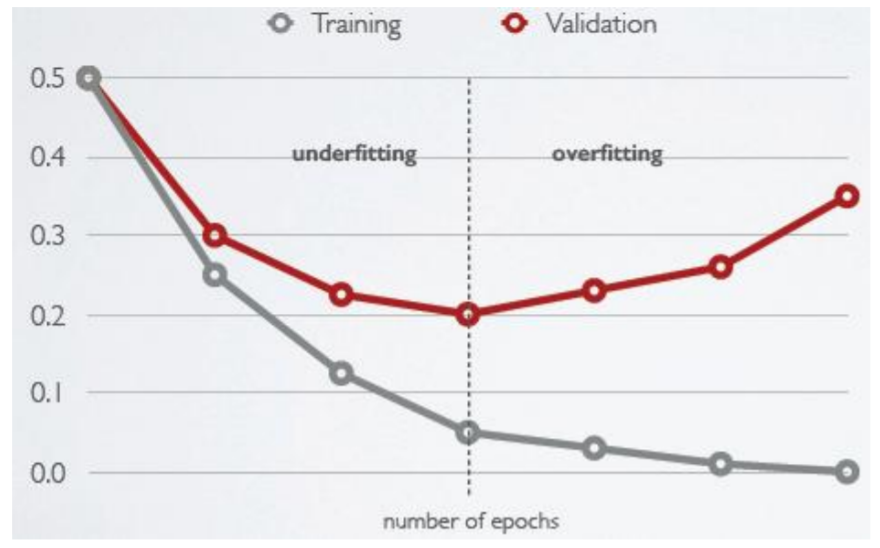
\includegraphics[scale=0.5]{figures/lear_rate.png}
	\caption{ Настройка темпа обучения }\label{fig:lear_rate}
\end{figure}

Увеличение размера пакета -- тот же эффект, что и уменьшение темпа обучения.

\subsection{Продвинутая оптимизация}

Стохастический градиент (надо случайно перемешивать данные перед каждой эпохой)
\begin{align*}
	w^{(t+1)} = w^{(t)} - \eta \, \nabla L^{(t)}(w^{(t)}).
\end{align*}

Стохастический градиент с моментом (Momentum)
\begin{align*}
	m^{(t+1)} = \rho \, m^{(t)} + \nabla L^{(t)}(w^{(t)}),\\
	w^{(t+1)} = w^{(t)} - \eta \, m^{(t+1)} = \underbrace{ w^{(t)} - \eta \, \nabla L^{(t)}(w^{(t)}) }_{\text{\itshape стохастический градиент}}+ \underbrace{- \eta \, \rho \, m^{(t)}}_{\text{\itshape добавление инерции}}.
\end{align*}

Метод Нестерова
\begin{align*}
	m^{(t+1)} = \rho \, m^{(t)} + \nabla L^{(t)} (w^{(t)} - \eta \, m^{(t)}),\\
	w^{(t+1)} = w^{(t)} - \eta \, m^{(t+1)} = w^{(t)} - \eta \, \nabla L^{(t)}(w^{(t)} + \underbrace{\color{blue} - \eta \, m^{(t)}}_{\text{\itshape\color{blue} смещение}}) + \underbrace{\color{blue} - \eta \, \rho \, m^{(t)} }_{\text{\itshape\color{blue} добавление инерции}}.
\end{align*}

\section{Графовые нейронные сети}

Полезные ресурсы Distill
\begin{itemize}
	\item \url{https://distill.pub/2021/understanding-gnns/},
	
	\item \url{https://distill.pub/2021/gnn-intro/}.
\end{itemize}


Графовые нейронные сети (GNN) вычисляют предаставления вершин в итеративном процессе, разные виды GNN по-разному, каждая итерация соответствует слою сети. Самая простая концепция такого вычисления -- неронное распространение (Neural Message Passing). Вообще, распространение сообщений довольно известный прием в анализе графов, заключается в том, что каждая вершина имеет некоторое состояние, которое за одну итерацию уточняется по следующей формуле
\begin{align*}
	h_v^{(k)} = \text{UPDATE}^{(k)} \Big( h_v^{(k-1)},  \text{AGG}^{(k)} (\{ h_u^{(k-1)} \}_{u \in N(v)}) \Big),
\end{align*}
где $ N(v) $ -- окрестной вершины $ v $, $ \text{AGG} $ -- функция аггрегации (по смыслу она собирает информацию о соседях, например, суммируя состояния), $ \text{UPDATE} $ -- функция обновления состояния вершины (с учетом собранной информации о сосдениях).

Единственное требование, которое накладывается на последние две функции -- дифференциируемость, чтобы использовать их в вычислительном графе и вычислять параметры сети методом обратного распространения.

\noindent\emph{Для графовых сверточных нейронных сетей}

\begin{align*}
	h_v^{(0)} = x_v, \ \forall v \in V,
\end{align*}
где $ h_v^{(0)} $ -- начальное представление узла $ v $, $ x_v $ -- оригинальные признаки узла $ v $.

И теперь для каждого шага $ k = 1, 2, \ldots, K $ [Distill]
\begin{align*}
	h_v^{(k)} = f^{(k)} \Big( W^{(k)} \cdot \dfrac{ \sum\limits_{ u \in N(v) } h_u^{(k-1)} }{ |N(v)| } + B^{(k)} \cdot h_v^{(k-1)}\Big), \ \forall v \in V,
\end{align*}
где $ h_v^{(k)} $ -- представление узла $ v $ на шаге $ k $, $ h_v^{(k-1)} $ -- представление узла $ v $ на шаге $ k - 1 $.

\remark{
Веса $ W^{(k)} $ и $ B^{(k)} $ разделяются между всеми узлами графа
}

Выражение справа от коэффициента $ W^{(k)} $ -- среднее представлений соседей вершины $ v $ на шаге $ k - 1 $.

Построить прогноз на каждом узле можно с помощью последнего вычисленного представления
\begin{align*}
	\hat{y}_v = \text{PREDICT}(h_v^{(K)}),
\end{align*}
где $ \text{PREDICT} $ -- как правило, другая нейронная сеть, обученная вместе с моделью GCN.

\remark{
GCN хорошо масштабируется, поскольку количество параметров в модели не привязано к размеру графа
}

Пример (\pic{fig:GCN}). Для вершины $ A $ на шаге 1 представление можно вычислить следующим образом, опросив соседей вершины
\begin{align*}
	h_A^{(1)} &= f\Big( W^{(1)} \times \dfrac{ h_E^{(0)} + h_F^{(0)} + h_G^{(0)} }{ 3 } + B^{(1)} \times h_A^{(0)} \Big) \\
	&= f(1 \times \dfrac{ 2 + (-2) + 0 }{ 3 } + 1 \times -4) \\
	&= f(0 + (-4)) \\
	&= f(-4) \\
	&= ReLU(-4) = 0.
\end{align*}

\begin{figure}[h]
	\centering
	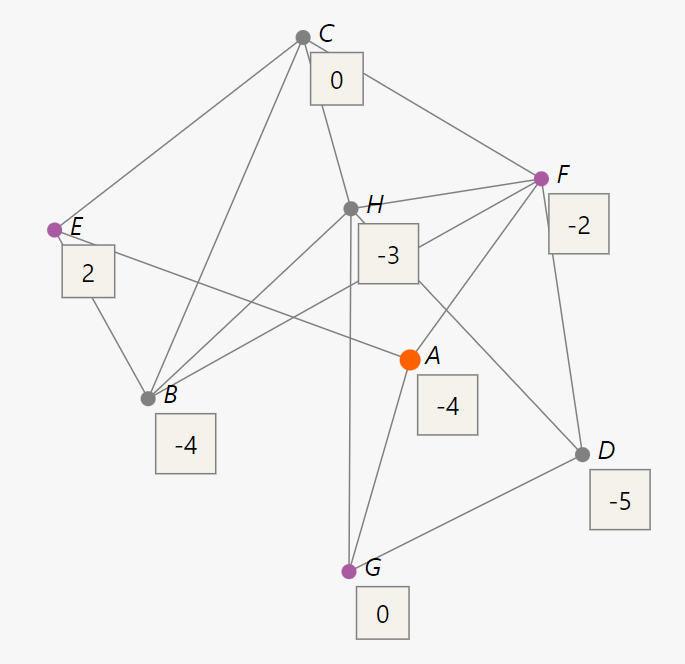
\includegraphics[scale=0.5]{figures/GCN.png}
	\caption{ Пример вычисления обновленного представления узла $ A $ на шаге 1 \\в графовой сверточной нейронной сети }\label{fig:GCN}
\end{figure}

На практике каждая описанная выше итерация обычно рассматривается как один <<слой нейронной сети>>. Этой идеологии придерживаются многие популярные библиотеки графовых нейронных сетей (PyTorch Geometic, StellarGraph), позволяющие создавать различные типы сверток графа в одной и той же модели.

Методы, которые мы рассматривали до сих пор, выполняют <<локальные>> свертки: признак каждого узла обновляется с использованием информации о признаках его локальных соседей. Однако можно построить и <<глобальную>> свертку.

После выбора произвольного порядка узлов мы можем собрать все признаки в вектор $ x \in \mathbb{R} $.

После нормализации $ x $ как $ \sum\limits_{i=1}^n x_i^2 = 1 $
\begin{align*}
	R_L(x) = \dfrac{ x^T Lx }{ x^T x} = \dfrac{ \sum_{(i,j) \in E} (x_i - x_j)^2 }{ \sum_i x_i^2 } = \sum_{ (i, j) \in E } (x_i - x_j)^2.
\end{align*} 

Множество собственных чисел лапласиана $ L $ называют \emph{спектром}. Спектральное разложение
\begin{align*}
	L = U \Lambda U^T, \ \Lambda = \text{diag}(\lambda_1, \ldots, \lambda_n), \ U = \{u_1 \ldots u_n\}, \ U^T U = I,
\end{align*}
где $ \Lambda $ -- диагональная матрица отсортированных собственных чисел, $ U $ -- обозначает матрицу собственных векторов, отсортированных по возрастанию собственных чисел.

Каждый вектор признаков $ x $ может быть представлен в виде линейной комбинации собственных векторов
\begin{align*}
	x = \sum_{i=1}^n \hat{x}_i u_i = U \hat{x},
\end{align*}
где $ \hat{x} $ -- это вектор коэффициентов $ [x_0, \ldots, x_n] $. Будем называть $ \hat{x} $ \emph{спектральным представлением} вектора признаков $ x $.

\remark{
Свертку в спектральной области графа можно рассматривать как обобщение свертки в частотной области изображений
}

Теория спектральных сверток математически обоснована, но есть несколько нюаносов:
\begin{itemize}
	\item Нам требуется вычислить матрицу собственных векторов $ U_m $. Для больших графов это неосуществимо,
	
	\item Даже если мы сможем вычислить $ U_m $, сами глобальные свертки неэффективны из-за повторяющегося умножения,
	
	\item Изученные фильтры специфичны для графов, поскольку они представлены в терминах спектрального разложения входного графа Лапласиана. Это означает, что они плохо переносятся на новые графы, которые имеют существенно иную структуру (и, следовательно, существенно разные собственные значения).
\end{itemize}

Хотя спекртальные свертки в значительной степени были вытеснены <<локальными>> свертками по рассмотренным выше причинам, все еще имеет смысл изучать идеи, лежащие в их основе.

Функции потерь для различных задач на графах:
\begin{itemize}
	\item Классификация узлов:
\begin{align*}
	\mathcal{L}(y_v, \hat{y}_v) = - \sum_c y_{vc} \log \hat{y}_{vc},
\end{align*}
где $ \hat{y}_{vc} $ -- предсказанная вероятность того что узел $ v $ принадлежит классу $ c $. GNNs адаптированы и для обучения на частично-размеченных данных, когда только некоторые узлы имеют разметку. В этом случае функцию потерь можно так
\begin{align*}
	\mathcal{L}_G = \dfrac{ \sum\limits_{ v \in \text{ Lab }(G) } \mathcal{L}(y_v, \hat{y}_v)}{ | \text{Lab}(G) | },
\end{align*}
где потери можно вычислить только на размеченных узлах $ \text{Lab}(G) $.

    \item Классификация графа: собрав информацию о представлении узлов графа, можно составить векторное представление графа. 
    
    \item Предсказание вероятности появления связи: опираясь на пары смежных и несмежных узлов, можно использовать их векторные представления в качестве входных данных для прогнозирования наличия / отсутствия связи
\begin{align*}
	\mathcal{L}(y_v, y_u, e_{vu}) = - e_{vu} \log (p_{vu}) - (1 - e_{vu}) \log(1 - p_{vu}),\\
	p_{vu} = \sigma (y_v^T y_u),
\end{align*}
где $ \sigma $ -- логистический сигмоид, и $ e_{vu} = 1 $, если между узлами $ v $ и $ u $ есть связь, и $ e_{vu} = 0 $ в противном случае.

    \item Кластеризация узлов: простая кластеризация представлений узлов.
\end{itemize}

Основная проблема при использовании описываемого нейронного распространения, т.н. \emph{чрезмерное сглаживание} (over-smoothing): после нескольких итераций пересчета состояний вершин представления соседних вершин становятся похожими, поскольку у них похожие окрестности. Для борьбы с этим делают
\begin{itemize}
	\item меньше слоев агрегации и больше для <<обработки признаков>>,
	
	\item прокидывание слоев или конкатенацию состояний с предыдущих слоев,
	
	\item используют архитектуры, в которых есть эффект памяти,
	
	\item приемы с номировками,
	
	\item используют аугментацию, например, DropEdge,
	
	\item используют noise regularization.
\end{itemize}

Сводка по графовым нейронным сетям
\begin{itemize}
	\item На вход сети подается граф, каждая вершина которого имеет признаковое описание. Это описание можно считать начальным состоянием вершины,
	
	\item Могут быть слои, которые независимо модифицируют представления (для каждой вершины его представление пропускается через небольшую нейронку),
	
	\item Могут быть слои, которые модифицируют представления всех вершин, учитывая представления вершин-соседей,
	
	\item Могут быть слои, упрощающие граф (например, уменьшающие число вершин),
	
	\item Могут быть слои, получающие представление графа (вектор фиксированной длины) по текущему графу с представлениями вершин.
\end{itemize}



\section{Отбор признаков с библиотекой BoostARoota}

BoostARoota \url{https://github.com/chasedehan/BoostARoota} -- алгоритм отобора признаков на базе экстримального градиентного бустинга в реализации XGBoost. Алгоритм требует гораздо меньших затрат времени на выполнение. Перед применением необходимо выполнить дамми-кодирование, поскольку базовая модель работает только с количественными признаками.

Отбор признаков выполняется на обучающем поднаборе данных, поэтому предполагается, что массив меток и массив признаков \emph{обучающие}, а для проверки качества модели отбора признаков есть независимая, \emph{тестовая} выборка. Кроме того, если необходимо выбрать оптимальные значения гиперпараметров модели отбора признаков (например, значения гиперпараметров \texttt{cutoff}, \texttt{iters} и \texttt{delta}), то понадобиться еще \emph{проверочная} {выборка}.

\section{Классический и байесовский бутстреп}

Бутстреп является универсальным инструментом для оценки статистической точности. 

Байесовский бутстреп это байевоский аналог классического бутстрапа. Вместо моделирования распределения выборки для статистики, оценивающей параметр, байесовский бутстреп моделирует \emph{апостериорное распределение параметра}. 

Основная идея состоит в том, чтобы случайным образом извлекать наборы данных с \underline{возвращением} из обучающих данных так, чтобы каждая выборка имела тот же размер, что и исходное обучающее множество.Это делается $ B $ раз (скажем, $ B = 100 $), создавая $ B $ множеств бутстрепа. Затем мы заново аппроксимируем модель для каждого из множест бутстрепа и исследуем поведение аппроксимаций на $ B $ выборках.

По выборке бутстрепа мы можем оценить любой аспект распределения $ S(\mathbf{Z}) $ (это любая величина, вычисленная по данным $ \mathbf{Z} $), например, его дисперсию
\begin{align*}
	\widehat{ Var }[ S(\mathbf{Z}) ] = \dfrac{1}{B - 1} \sum_{b=1}^{B} \Big( S(\mathbf{Z}^{*b})  - \bar{S}^* \Big)^2, \quad \bar{S}^{*} = \sum_b S( \mathbf{Z}^{*b} ) / B.
\end{align*}

\section{HDI}

Highest Density Interval (HDI) -- интервал высокой плотности -- показывает какие точки распределения наиболее достоверны/правдоподобны и охватывают большую часть распределения. Каждая точка внутри интервала имеет более высокую \emph{достоверность}, чем любая точка вне интервала.

\section{Площадь по ROC-кривой}

Построение ROC-кривой происходит следующим образом (\pic{fig:roc_auc0}):
\begin{enumerate}
	\item  Сначала сортируем все наблюдения по убыванию спрогнозированной вероятности положительного класса,
	
	\item Берем единичный квадрат на координатной плоскости. Значения оси абсцисс будут значениями 1 - специфичности (цена деления оси задается значением 1/neg), а значения оси ординат будут значениями чувствительности (цена деления оси задается значением 1/pos). При этом pos — это количество наблюдений положительного класса, а neg — количество наблюдений отрицательного класса,
	
	\item Задаем точку c координатами (0, 0) и для каждого отсортированного наблюдения x:
	\begin{itemize}
		\item если x принадлежит положительному классу, двигаемся на 1/pos вверх,
		
		\item если x принадлежит отрицательному классу, двигаемся на 1/neg вправо.
	\end{itemize}
\end{enumerate}

Значение вероятности положительного класса, при котором ROC-кривая находится на минимальном расстоянии от верхнего левого угла -- точки с координатами (0, 1), дает наибольшую правильность классификации. В данному случае (\pic{fig:roc_auc0-1}) будет 0.72.

\begin{figure}[h]
	\centering
	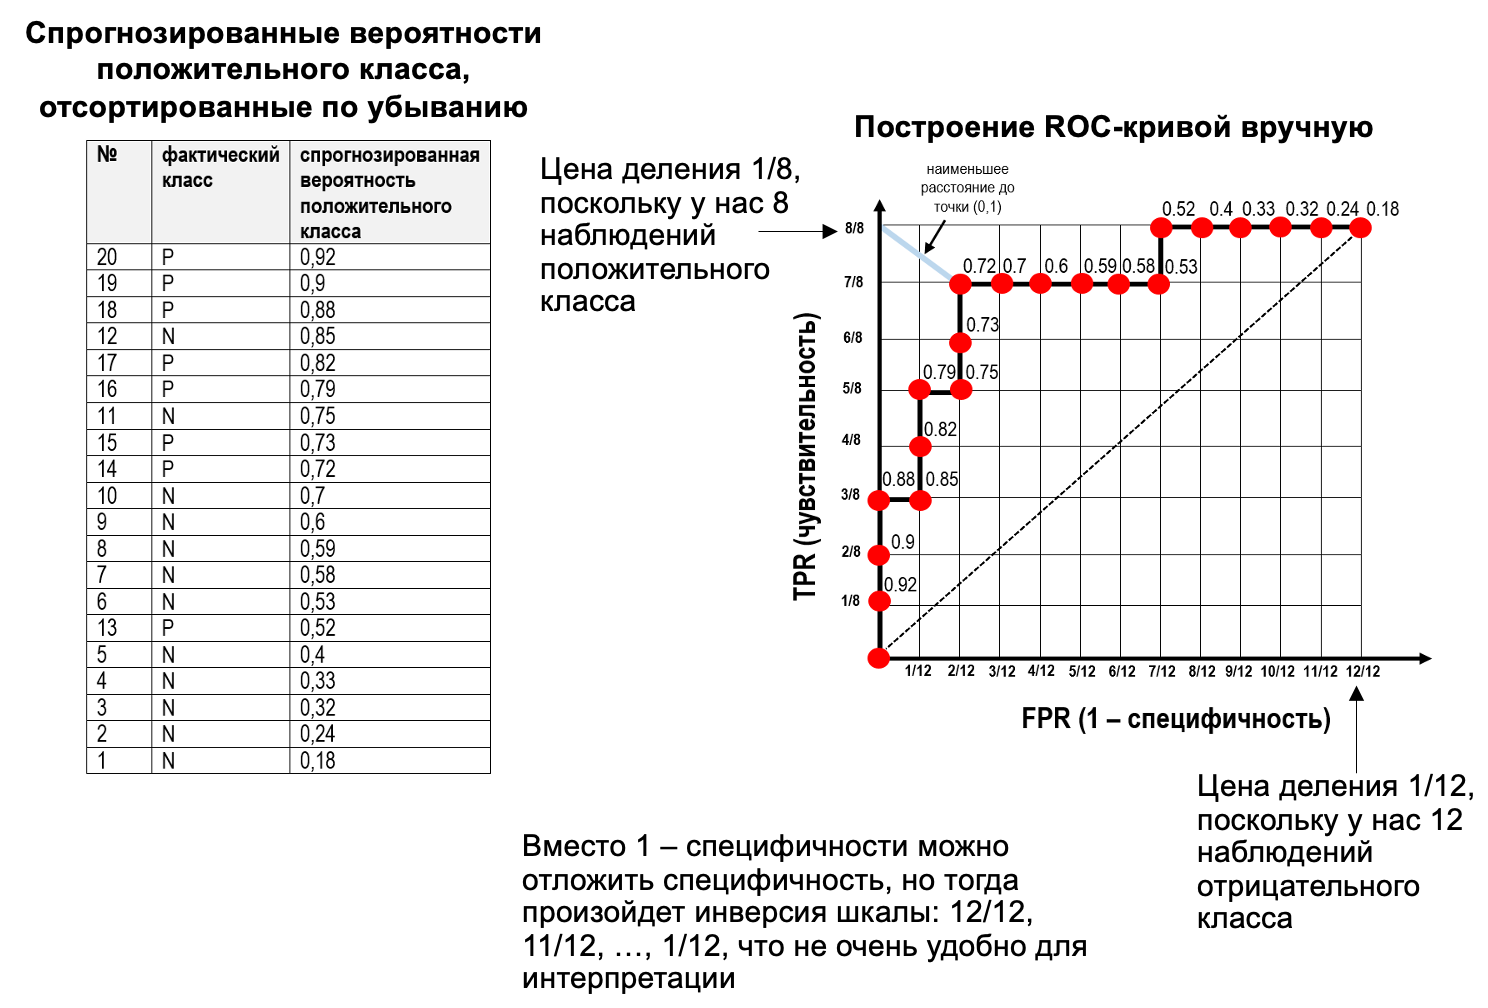
\includegraphics[scale=0.3]{figures/roc_auc0.png}
	\caption{ Построение ROC-кривой }\label{fig:roc_auc0}
\end{figure}

\begin{figure}[h]
	\centering
	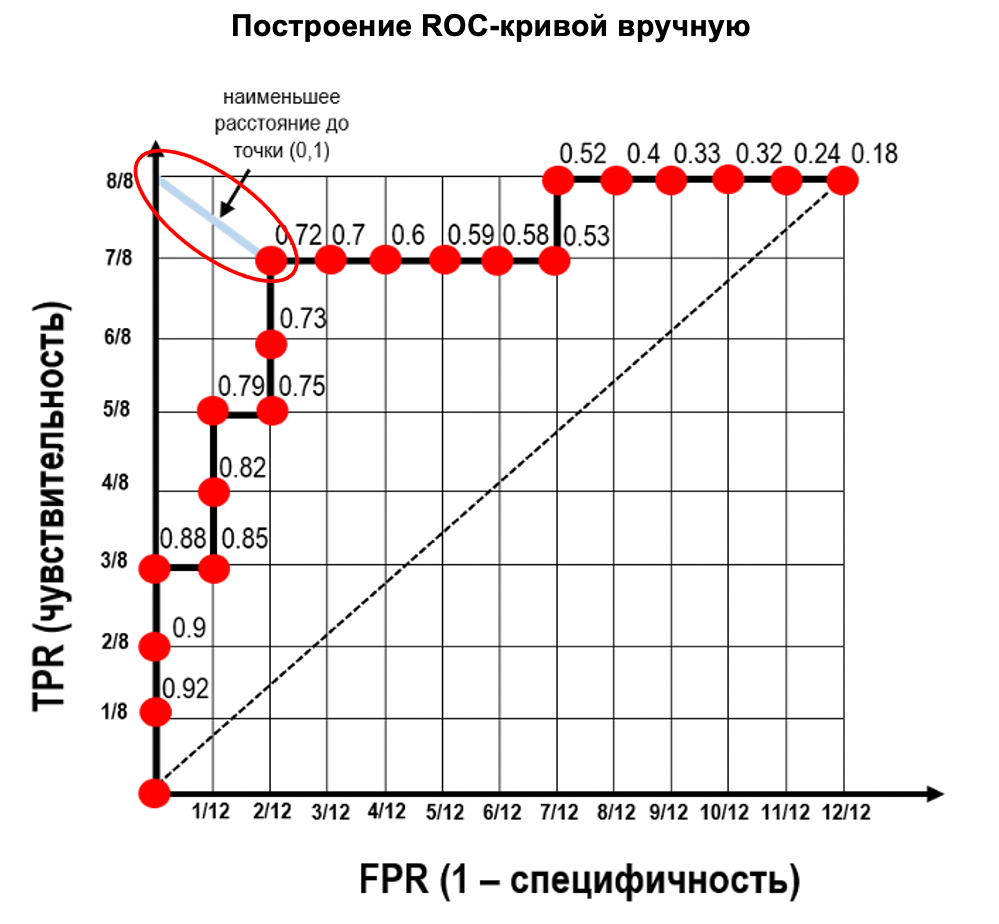
\includegraphics[scale=0.3]{figures/roc_auc0-1.png}
	\caption{ ROC-кривая. Порог отсечения 0.72 }\label{fig:roc_auc0-1}
\end{figure}

Площадь под ROC-кривой (ROC-AUC) можно интерпретировать как вероятность события, состоящего в том, что классификатор присвоит более высокий ранг (например, вероятность) случайно выбранному экземпляру положительного класса, чем случайно выбранному экземпляру отрицательного класса (если не рассматривать вариант равенства значений рангов).

\remark{
На ROC-кривые не влияет баланс классов (при достаточном объеме выборки) и они могут чрезмерно оптимистично оценивать качество работы алгоритма в случае дисбалансов. Лучше пользоваться гармоническим средним или PR-кривыми
}

Однако недостаток такой интепретации заключается в том, что мы пренебрегаем часто встречающейся ситуацией равенства вероятностей. Поэтому правильнее будет сказать, что ROC-AUC равен доле пар вида (экземпляр положительного класса, экземпляр отрицательного класса), которые алгоритм верно упорядочил в соответствии с формулой
\begin{align}\label{eq:rocauc}
	\dfrac{ \sum\limits_{i, j=1}^{n_i, n_j} s(x_i, x_j)}{ n_i \, n_j }, \quad s(x_i, x_j) =
	\begin{cases}
		1, x_i > x_j,\\
		1/2, x_i = x_j,\\
		0, x_i < x_j,
	\end{cases}
\end{align}
где $ x_i $ -- ответ алгоритма для положительного экземпляра, $ x_j $ -- ответ алгоритма для отрицательного экземпляра.

По сути числитель дроби представляет собой сумму количеств $ j $-ых наблюдений отрицательного класса, лежащих ниже каждого $ i $-ого наблюдения положительного класса. Каждое такое количество мы берем по каждому $ i $-ому наблюдению положительного класса в последовательности, отсортированной по мере убывания вероятности положительного класса. Знаменатель дроби -- это произведение количества наблюдений положительного класса и наблюдений отрицательного класса.

Если говорить более точно, мы берем наблюдение положительного класса под номером 20 и каждый раз образовываем пару с наблюдением отрицательного класса (\pic{fig:roc_auc1}), у нас 12 пар, 12 раз наблюдение полжительного класса под номером 20 было проранжировано выше наблюдений отрицательного класса 12, 11, 10 и т.д. Записываем число 12 напротив наблюдения 20. 

Разные модели нельзя сравнивать только по ROC-AUC. ROC-AUC оценивает разные классификатор, используя метрику, которая сама зависит от классификатора. То есть ROC-AUC оценивает разные классификаторы, используя разные метрики.

\remark{
Если часть ROC-кривой лежит ниже диагональной линии, а часть -- выше, то это означает, что классы не являются линейно-сепарабельными, а при этом используется линейная модель
}

При одинаковой ROC-AUC у разных моделей (соответственно с разными ROC-кривыми) будет разное распределение стоимостей ошибочной классификации. Проще говоря, мы можем вычислить ROC-AUC для классификатора A и получить 0.7, а затем вычислить ROC-AUC для второго классификатора и снова получить 0.7, но это не обязательно означает, что у них одна и та же эффективность.

\section{Приемы работы с Gurobi}

Полезный ресурс \url{https://www.gams.com/latest/docs/S_GUROBI.html#GUROBI_GAMS_GUROBI_LOG_FILE}

Чтобы запустить Gurobi в интерактвином режиме, следует в командной оболочке набрать \texttt{gurobi}
\begin{lstlisting}[
title = {\sffamily Сессия GUROBI},
style = bash,
numbers = none
]
gurobi> m = read("./ikp_milp_problem.lp")
gurobi> m.optimize()
gurobi> vars = m.getVars()
gurobi> help(m)
# вывести 2-картежи целочисленных переменных с отличным от нуля значением
gurobi> [(var.varName, var.x) for var in vars if (var.x > 0) and (var.vType == "I")]
gurobi> m.write("res.sol")  # записать решение
\end{lstlisting}


\begin{figure}[h]
	\centering
	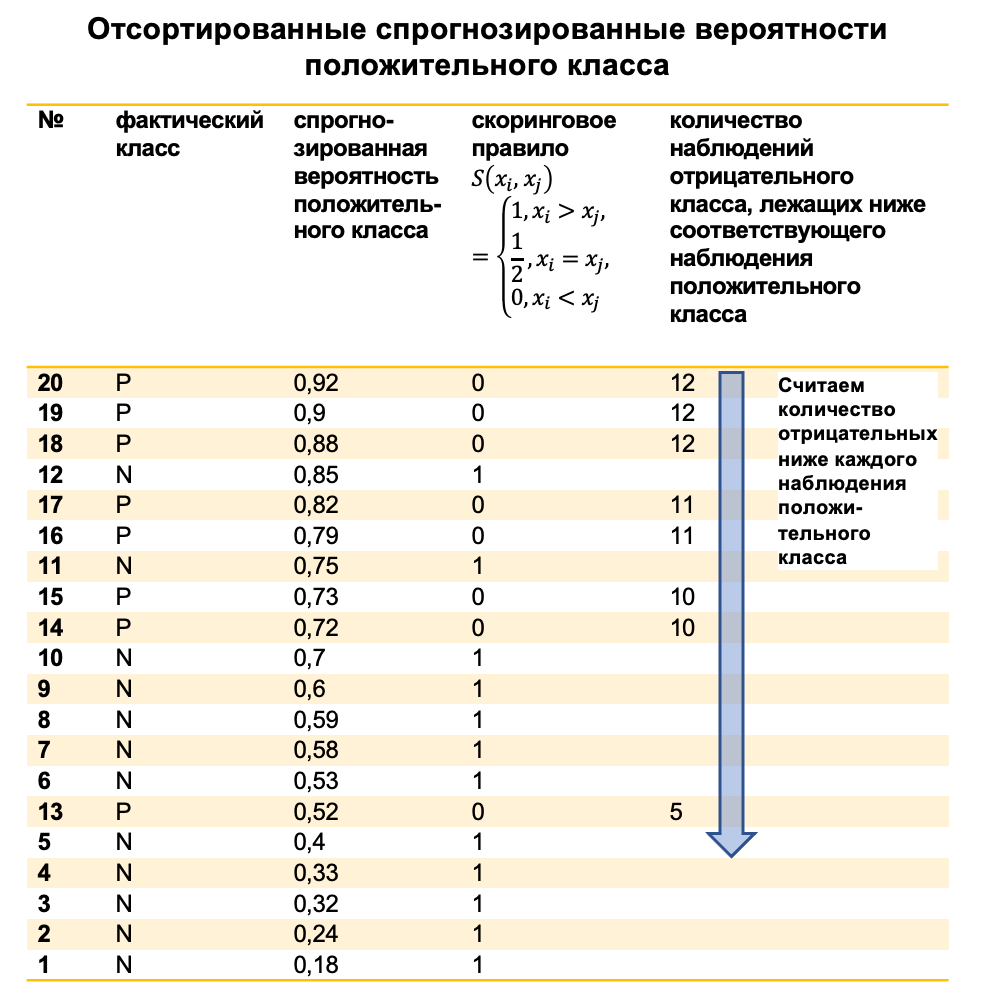
\includegraphics[scale=0.35]{figures/roc_auc1.png}
	\caption{ Расчет ROC-AUC по формуле \eqref{eq:rocauc}}\label{fig:roc_auc1}
\end{figure}

\begin{figure}[h]
	\centering
	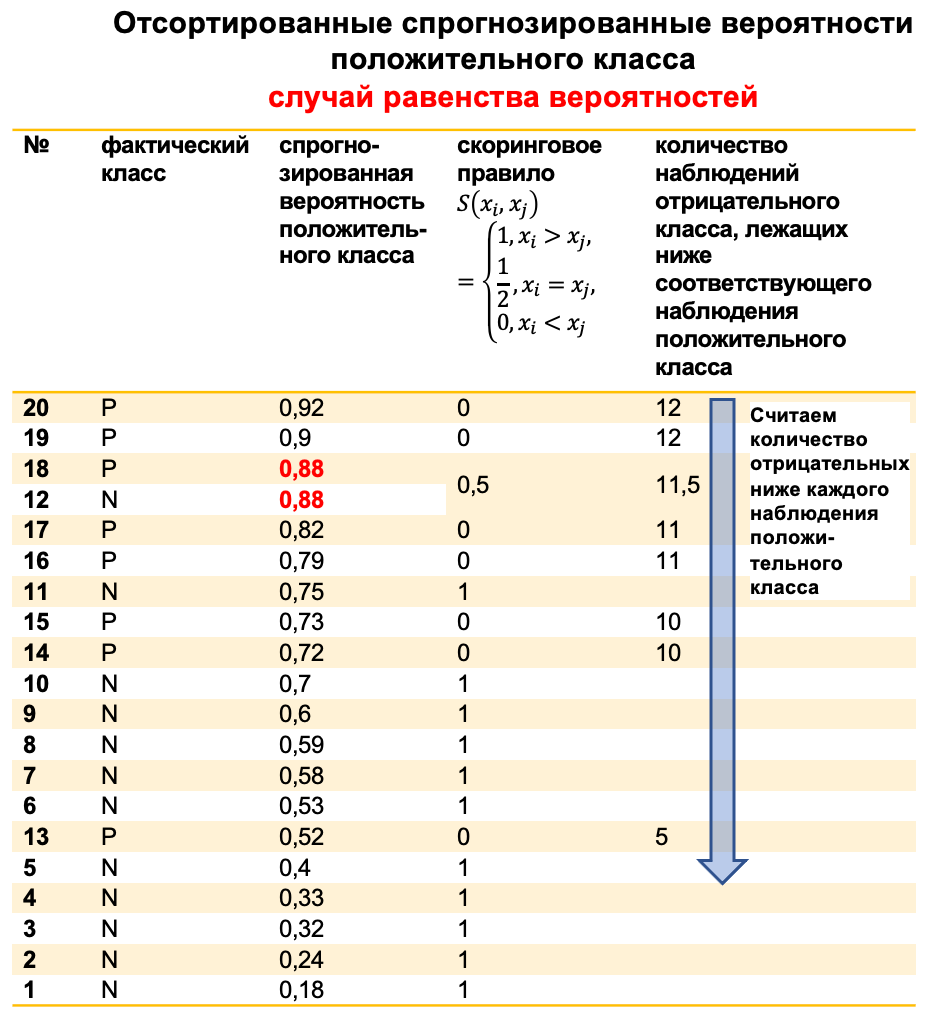
\includegraphics[scale=0.35]{figures/roc_auc2.png}
	\caption{ Расчет ROC-AUC по формуле \eqref{eq:rocauc} для случая равных вероятностей принадлежности экземпляра положительному классу}\label{fig:roc_auc2}
\end{figure}




\listoffigures\addcontentsline{toc}{section}{Список иллюстраций}

% Источники в "Газовой промышленности" нумеруются по мере упоминания 
\begin{thebibliography}{99}\addcontentsline{toc}{section}{Список литературы}
	\bibitem{lutz:learningpython-2011}{\emph{Лутц М.} Изучаем Python, 4-е издание. -- Пер. с англ. -- СПб.: Символ-Плюс, 2011. -- 1280~с. }
		
	\bibitem{beazley:python-2010}{\emph{Бизли Д.} Python. Подробный справочник. -- Пер. с англ. -- СПб.: Символ-Плюс, 2010. -- 864~с. }
\end{thebibliography}

\end{document}
